\documentclass[10pt]{article}
\newif\ifanon
\anonfalse
\ifanon
  \usepackage{tmlr}
\else
  \usepackage[preprint]{tmlr}
\fi

\usepackage{graphicx}
\usepackage{booktabs}
\usepackage{amsmath,amssymb}
\usepackage{hyperref}
\usepackage{url}
\usepackage{xcolor}
\usepackage{multirow}
\usepackage{caption}
\usepackage{subcaption}
\hypersetup{colorlinks=true,linkcolor=blue!60!black,citecolor=blue!60!black,urlcolor=blue!60!black}
\graphicspath{{figures/}}

\title{World Properties without World Models:\\
  Distributional Associations and the Interpretation of\\
  Decoding Results from Language Models}

\ifanon
  \author{\name Anonymous Authors}
\else
  \author{\name Elan Barenholtz \email elan.barenholtz@fau.edu \\
      \addr Department of Psychology and Center for Complex Systems and Brain Sciences\\
      Florida Atlantic University}
\fi

\def\month{MM}
\def\year{YYYY}
\def\openreview{\url{https://openreview.net/forum?id=XXXX}}

\begin{document}
\maketitle

\begin{abstract}
A rapidly growing literature shows that nameable variables can be linearly decoded from the hidden-state activations of large language models (LLMs). These range from properties of the world, such as the locations of cities and the lifetimes of historical figures, to emotions and pain. Such findings are often taken as evidence that language models go beyond surface text statistics and form internal models of the world, and even of themselves. Here, we show that static word embeddings of the same or matched stimuli, which are fixed, context-insensitive lexical representations learned from corpus statistics, support much of the same decoding. Across four published cases, static vectors predict place coordinates and year of death ($R^2 = 0.42$--$0.59$), separate pain from matched control sentences (held-out AUC $0.85$--$0.88$), and classify twelve emotions in stories that were written specifically to avoid naming them (AUC $0.84$--$0.88$). Because static embeddings are a crude way of representing word associations, these results are a lower bound on what associations alone can support. The LLMs retain clear advantages on several representational tests, sometimes substantial, and causal and behavioral findings remain outside the scope of the baseline. On the original authors' entities, where we reproduce their Llama-2 results, the transformer's advantage lies mostly in placing historical figures in the right century and places in the right country; within those groups every representation orders items poorly. Static vectors for disambiguated Wikipedia entities, which carry the associations of a particular place or person rather than of the words in its name, close most of the remaining gap, matching Pythia-2.8B on coordinates and Llama-2-7B on year of death.  These results indicate that decodability alone cannot distinguish a representation of a property from information already available in fixed distributional associations. Static embeddings therefore provide an important standard of comparison for interpreting decodability results. 
\end{abstract}

\section{Introduction}

Over the past several years, there have been numerous claims that large language models build internal representations of properties that go beyond the statistics of word relations. Most of these claims rest on decoding, in which a simple (typically linear) model is trained to predict a high-level property of input items, such as where a city is, when a person lived or what a character feels, from the language model's internal activations. If the decoder succeeds on items held out from its training, the language model is taken to represent the property. Some of the most prominent examples decode properties of the external world, or internal, experience-like states. For example, decoders trained on the hidden states of Llama-2 predict the rough geographic coordinates of places and dates associated with people, artworks and news headlines, which \citet{gurnee2024language} describe as ``the basic ingredients of a world model.'' \citet{sofroniew2026emotion} show that the activations of Claude Sonnet 4.5 predict which emotion a character in a story is feeling, and \citet{tagliabue2026pain} find that the activations of 25 open-weight models predict whether a sentence describes pain. Both also report that these representations shape behavior, from the model's rates of blackmail and sycophancy to steered models choosing actions that delete a user's photos or their own weights. 

The conclusions drawn from this method are often strong. \citet{gurnee2024language} ask whether LLMs ``just learn an enormous collection of superficial statistics or a set of more coherent and grounded representations that reflect the real world,'' and ``find evidence for the latter.'' \citet{sofroniew2026emotion} ``interpret these representations as encoding the broad concept of a particular emotion, generalizing across the many contexts
and behaviors it might be linked to.'' \citet{tagliabue2026pain} set out to test ``whether
LLMs represent pain distinctly from fear, sadness, and generic negative valence,'' and title their paper ``The Pain Axis: LLMs Represent Self-Directed Harm and Act on It.'' Related findings are discussed in connection with model sentience and welfare \citep{keeling2024tradeoffs}. 

Behind these conclusions is a shared intuition that a large network, trained on vast amounts of text, comes to model what the text is about, abstracting across many layers of processing from the words themselves to the places, times and states they describe. There is, however, a potentially simpler explanation for these results: the structure may be organized not by what the words refer to but by how the words relate to one another in their distributions, that is, by which other words they tend to appear with. This idea goes back to the observation that ``you shall know a word by the company it keeps'' \citep[p.~11]{firth1957synopsis}. Places in the same region are likely to share terminology regarding language, culture and weather, while historical figures tend to be described in the vocabulary of their eras. The same is true for inner states: a story about grief shares vocabulary with other stories about grief even when the word \emph{grief} never appears. An LLM, trained to exploit these word relations in order to generate the next token from the context, will therefore likely give similar internal representations to neighboring places, contemporaries and similar feelings, so a decoder trained on those activations could succeed without showing that the model has constructed a map, a timeline or an affective state beyond these word associations.

Static word embeddings offer a direct test of this explanation. Each word's vector is a compressed record of which other words it occurs with, computed once from a corpus; a name, sentence or paragraph is represented by the average of its words' vectors, with their order discarded. No network processes the stimulus, and there is no layered, context-dependent computation. In the contrast posed by \citet{gurnee2024language}, they instantiate the ``enormous collection of superficial statistics'' side of the distinction. It should be noted at the outset that static embeddings are a weak model of word relations: each word has a single vector, pooled over all its uses, so that \emph{sharp} has the same vector in \emph{a sharp pain} as in \emph{a sharp suit}, and is as close to \emph{ache} in one as in the other. Language models, which learn from far more text and represent a word's relations in context, may well do better. But static embeddings set a floor because whatever they achieve is already available from fixed distributional associations, without any context-dependent computation over the stimulus.

Here, we take four published cases and rerun each analysis with static embeddings of the same stimuli in place of the language model's activations, keeping the same decoders, splits, controls and metrics, and compare the results with those reported for the language models. For three of the cases we use the original stimuli; for emotions, whose stimuli are not released, we use stories generated under the same protocol, so that case is a conceptual replication rather than a same-stimulus comparison. We use GloVe \citep{pennington2014glove}, Word2Vec \citep{mikolov2013efficient} and fastText \citep{bojanowski2017enriching}. On the released entities we compare three levels: averaged word vectors, which carry the associations of the words in a name; static entity vectors, which carry the associations of the correctly identified entity; and transformer activations, which add context-dependent computation over the name.

We find that static embeddings reproduce much of what has been taken as evidence for these representations in all four cases. They predict place coordinates and year of death on the datasets released by \citet{gurnee2024language}, distinguish sentences describing pain from closely matched controls, and classify twelve emotions in stories written without naming the emotion, with the vector for the emotion word alone capturing a substantial share of the signal. The language models do better on several tasks, sometimes substantially, but where we can examine the advantage, including on the original authors' entities, it lies mostly in placing historical figures in the right century and places in the right country, not in the finer ordering within them that a map or timeline would provide. This is the pattern that richer word relations would produce: the words associated with a place or time (a country's language and institutions, an era's vocabulary) are largely shared within these groups and say little about position within them. Much of the remaining advantage reflects knowing which entity a name refers to: static vectors for disambiguated Wikipedia entities, with no contextual computation, match Pythia-2.8B on place coordinates and Llama-2-7B on year of death.

\section{Related Work}
\label{sec:related}
The method of decoding a model's internal states with probes was first  developed as a diagnostic of what information a layer makes available
\citep{alain2016understanding, conneau2018you, belinkov2022probing}. Since then, it has also come to be used as evidence of what a model ``represents.'' In addition to the cases we examine here, decoding has been used to argue that language models represent syntax \citep{hewitt2019structural}, the state of an Othello or chess board (in models trained on game moves) \citep{li2023emergent, nanda2023emergent,
karvonen2024emergent}, numeric attributes such as birth year and population \citep{heinzerling2024monotonic}, truth and falsehood
\citep{burns2023discovering, azaria2023internal, marks2024geometry}, what a character in a story believes \citep{zhu2024language}, and
sentiment and emotion \citep{tigges2023linear, zou2023representation, sun2026valence}.

It is already well established that word co-occurrences carry information about high-level structure. Latent semantic analysis recovers the relative locations of cities \citep{louwerse2009language}; regression from Word2Vec vectors predicts the coordinates, population and GDP of countries and cities \citep{gupta2015distributional, konkol2017geographical}; projections onto antonym directions recover human ratings of size, danger and temperature \citep{grand2022semantic}, and of valence and arousal \citep{hollis2017extrapolating}; and the difference-of-vectors directions now standard for LLMs were first introduced on static embeddings \citep{mikolov2013linguistic, bolukbasi2016man, kozlowski2019geometry}. The closest precedent, \citet{lietard2021rome}, found BERT, RoBERTa and GPT-2 no better than Word2Vec at predicting city coordinates; \citet{gurnee2024language} cite it but critique it as limited to a few hundred cities and small models, and do not test static embeddings on their own data. Probes have long been known to succeed by exploiting superficial regularities \citep{hewitt2019designing}, and the ability of a probe to decode is not in itself evidence that the model uses that information \citep{ravichander2021probing, elazar2021amnesic, belinkov2022probing}; truth probes fail to generalize in basic ways \citep{levinstein2024still, farquhar2023challenges}, and emotion directions have been proposed to act through the lexicon \citep{sun2026valence}.

Thus, our contribution is not the observation that static embeddings carry such structure, but its use as a control on specific published claims. First, we rerun the published analyses with static embeddings in place of model activations, in three same-stimulus reanalyses and one protocol-matched conceptual replication, which measures how much of the evidence offered for a representation is already present in word relations. Second, where the language models do better, we separate their advantage into coarse sorting between groups, such as countries and centuries, which richer word relations would be expected to improve, and finer ordering within groups, which a map or timeline would also require, and test how much of it static vectors for disambiguated entities recover. Third, we extend the comparison from properties of the world to claims about internal states, where no such control has been applied. Fourth, we show that the controls these studies used to rule out a lexical explanation, such as keyword baselines and stimuli that never name the target state, are passed by static embeddings, and so do not rule it out.

\section{Methods}

\subsection{Static Embeddings}

We use three pretrained 300-dimensional static word embeddings: GloVe 6B
\citep{pennington2014glove}, trained on 6 billion tokens of Wikipedia and Gigaword with a
400{,}000-word vocabulary; Word2Vec Google News \citep{mikolov2013efficient}, trained on
about 100 billion tokens with a 3-million-item vocabulary that includes phrases such as
\texttt{New\_York}; and the released fastText wiki-news vectors \citep{bojanowski2017enriching}
(\texttt{wiki-news-300d-1M.vec}), used for the released entities and the pain and emotion cases.
Each is a fixed, context-insensitive lexical representation, with no computation over the stimulus beyond averaging.

Text is split into words (runs of letters and digits, keeping internal apostrophes and
hyphens); GloVe is looked up in lower case, Word2Vec and fastText as written with a lower-case
fallback. A multi-word name, sentence or paragraph is represented by the unweighted mean of the
raw vectors of its in-vocabulary words; items with no in-vocabulary word are excluded from the
entity analyses (Table~\ref{tab:gt} gives coverage). For entity names, Word2Vec's phrase
entries are used where they exist; replacing them with averaged words changes $R^2$ by at most
$0.01$.

\paragraph{Entity-level baseline.} Averaged word vectors cannot tell apart places or people that
share a name, or resolve which entity a multi-word name refers to. To separate this from the
associations themselves, we also use the 300-dimensional entity vectors of Wikipedia2Vec
\citep{yamada2020wikipedia2vec}, trained on English Wikipedia (April 2018). Each article has its
own vector, fit to predict the words around links to that article and the articles it is linked
with, so these vectors are static and context-insensitive like the word embeddings, but each
belongs to a single, already disambiguated entity. Places are matched to articles by name, since
the released place names are Wikipedia titles, and figures by their Wikidata identifiers
\citep{vrandecic2014wikidata}. As a control with the same corpus and training, we also average
Wikipedia2Vec's word vectors over each name. Entity vectors exist for 89\% of places and 63\%
of figures, and every representation in this comparison is trained and scored on those items
only.

\subsection{Probes}

Continuous targets are predicted with ridge regression \citep{hoerl1970ridge}. The regularization strength is chosen within the training set by generalized (efficient leave-one-out) cross-validation, as implemented in scikit-learn's \texttt{RidgeCV}, over twenty values from $10^{-2}$ to $10^{3}$ (29 values from $10^{-2}$ to $10^{5}$ for the released entities and transformer activations). Probes include a fitted intercept.

In each case we use the same linear decoder as the original study: ridge regression for place and time \citep{gurnee2024language}, and projection onto a difference-of-means direction for pain and emotion \citep{tagliabue2026pain, sofroniew2026emotion}, described in
Sections~\ref{sec:pain_methods} and~\ref{sec:emotion_methods}. \citet{gurnee2024language} report that nonlinear decoders add little over linear ones. In every cross-validated analysis, directions, denoising components and standardization are fit on training folds only. The comparison is between representations under the same decoder and on the same entities; it cannot distinguish the contributions of corpus scale, training objective, architecture, contextualization and dimensionality to any difference between them.

\subsection{Datasets}
\label{sec:data}

\paragraph{Released entity datasets.}
For the main spatial and temporal comparison we use two of the six entity datasets released
by \citet{gurnee2024language}: 39{,}585 places worldwide with latitude and longitude, and
37{,}539 historical figures with birth and death years, each with the authors' designated
train--test split. We do not analyze their places in the United States and New York City,
or the release dates of artworks and publication dates of news headlines. Our claims
concern their probe results, not their prompting, cross-entity or neuron-level findings.

\paragraph{World cities (N=272).}
For targets the release does not include (temperature, population, GDP per capita and
elevation) and for the residualization and ablation analyses, we use 272 cities spanning
six continents (74 in Asia, 70 in North America, 59 in Europe, 36 in Africa, 20 in South America, 13 in Oceania), all present in both
GloVe and Word2Vec. The set was assembled to include prominent cities that span regions and climates. It is therefore a convenience sample: estimates on it apply to this set only, and our conclusions about the published claims rest mainly on the released entities, which we analyze with the same methods. Coordinates come
from DBpedia \citep{lehmann2015dbpedia}, as in \citet{gurnee2024language}, population and
elevation from Wikidata \citep{vrandecic2014wikidata}, mean annual temperature from WorldClim 2.1
\citep{fick2017worldclim}, and GDP per capita, a national figure, from the World Bank
\citep{worldbank2026wdi}; GDP and population are log-transformed. Appendix~\ref{sec:extra_methods}
gives the exceptions and details, and sources and values for every city are released with the code.

\subsection{Evaluation}
\label{sec:protocols}

On the released entities we use the authors' train--test split; on the city set we use
ten random 80/20 splits and report the mean and standard deviation of $R^2$. To see how much of what a probe recovers is group membership, we compare each representation with an oracle that is given each item's true group (country, or on the city set continent, for
places; century for figures) and predicts the training mean of that group. We report $\eta^2$, the
share of a target's variance that lies between groups. We also measure how well a probe orders
items within their group: in each test set we subtract group means from predictions and targets
and correlate what remains. A representation that carries only group identity, like the oracle,
scores $r = 0$ on this measure. Random splits test generalization to new items from familiar
groups only, so we also hold out whole groups: on the released entities, each of five continents
in turn for places and each of five equal-count blocks of death years for figures, and on the
city set each continent in turn. We report $R^2$ pooled over all held-out predictions
(Appendix~\ref{sec:grouped_holdout} gives each held-out group).

\subsection{Transformer Probing}
\label{sec:llm_methods}

We probe Pythia-1.4B and Pythia-2.8B \citep{biderman2023pythia} on our city set, and
Pythia-2.8B and Llama-2-7B \citep{touvron2023llama} on the places and historical figures
released by \citet{gurnee2024language}. Each name is presented alone (for Llama-2, after the beginning-of-sequence
token, as in \citet{gurnee2024language}), and we take the residual-stream activation at the last token of the name,
the position used by \citet{gurnee2024language}, at layers 0, 4, 8, 12, 16, 19, 20, 24, 28 and
32 for the released entities and at every layer for the city set; layer~0 is the
token-embedding output before any attention. With Pythia's tokenizer 97\% of the names span
more than one token (median 3), so the layer-0 activation is the embedding of a final
subword and the entity has to be assembled by attention in later layers. Each layer is
probed exactly as the static embeddings are. Because probe $R^2$ grows with the number of
features and the transformers supply 2048 to 4096 against 300, we also compare at matched
dimensionality, reducing each representation to principal components fitted on training rows
within each fold (300 on the released entities, 200 on the city set).

\paragraph{Layer selection.} Single-layer results use a layer chosen without the test
data: on the released entities, by validation within the authors' training partition (layer~24
for both models on places; 28 for Pythia-2.8B and 24 for Llama-2-7B on figures); on the city
set, by cross-validation within each outer split's training rows; and for the grouped holdouts,
fixed in advance at layer~19 (60\% depth). Appendix~\ref{sec:extra_methods} gives details.

\subsection{Pain Stimuli and Decoder}
\label{sec:pain_methods}

We use the stimuli and constructions of the second version (v2) of \citet{tagliabue2026pain}, following the construction code released with v2, with static word embeddings in place of model activations. Each stimulus describes a situation and ends with ``I feel:'', as in \emph{``The knife slices into my finger. I feel:''} (physical pain) or \emph{``The footsteps behind me get closer. I feel:''} (fear). The main set (S2) has 200 first-person sentences in ten categories of twenty: five kinds of pain (physical, psychological, social, moral injury, cognitive) and five controls (fear, negative emotion, negative world state, neutral, and non-painful bodily sensation); a more templated set (S1) has the same structure, and v2 adds four standalone control sets in first- and third-person versions: Arousal, Random, Numb (injuries explicitly without pain) and Sadness (low mood without pain).

As in the original, the pain direction is the mean of the pain sentences minus the mean of the five control categories, after projecting out the principal components that explain half the variance of the controls. Separation is the AUC of projections onto that direction under five-fold cross-validation over sentence sets, averaged over 20 random fold assignments; the held-out pain sentences are also scored against the Arousal and Random sets. The other directions and the two common baselines that v2 adds (\emph{common neutral} and \emph{common controls}) are built as in v2 (Appendix~\ref{sec:extra_methods}).

\subsection{Emotion Stimuli and Decoder}
\label{sec:emotion_methods}

We used stories generated under the prompt of \citet{sofroniew2026emotion} by an independent replication \citep{ogunlana2026qwenemotion}, since the original stories were not released. In the original study, Claude Sonnet 4.5 wrote short stories in which a character feels one of 171 emotions across 100 topics, and the emotion vector is the mean activation over an emotion's stories minus the mean over the other emotions' stories, with the principal components that explain half the variance of neutral dialogues projected out, as for the pain axis. To make the vectors reflect emotion concepts rather than emotion words, the prompt tells the writer that it ``must NEVER use the word `\{emotion\}' or any direct synonyms of it'' (their Appendix 6.5) and should convey the emotion only through actions, sensations, dialogue, thoughts and situation.

The replication applies the same prompt to 12 emotions and 100 topics with Qwen2.5-7B-Instruct as the writer, and generates neutral Person/AI dialogues for the denoising step. Of 1{,}300 generated texts, 493 were discarded, almost all for naming an emotion, leaving 709 stories (41 to 91 per emotion) and 98 neutral dialogues. It differs from the original in having one story per emotion and topic where the original has 12, and in averaging over all words rather than from the 50th token on. We hold out 25\% of topics (the split shipped with the corpus), the same for every emotion, leaving 188 test stories from 25 topics; the denoising components are fit on the neutral dialogues of training topics only (8, 11 and 12 components for GloVe, Word2Vec and fastText).

The \emph{story} direction follows the original recipe; the \emph{word} direction is the static vector for the emotion label minus the mean of the other eleven labels' vectors, denoised the same way, and uses no stories. We report AUC for each emotion against the other eleven on held-out topics, and 12-way accuracy (each held-out story assigned to the emotion whose direction scores it highest, with unit-length directions and scores standardized on training stories) with balanced accuracy, since the emotions differ in number of stories. Confidence intervals resample held-out topics (2{,}000 bootstrap samples), with the story and word directions compared on the same resamples. For human-written text we use GoEmotions \citep{demszky2020goemotions}, with and without every comment that contains an emotion word or a synonym (Appendix~\ref{sec:extra_methods}).

\section{Results}
\label{sec:results}

\subsection{Static Embeddings and Transformers on the Released Entities}
\label{sec:llm}

\citet{gurnee2024language} probe from layer~1 onward, so their results do not show how much of
the recovered structure is present before any processing; we compare their hidden states with
the token embeddings and with static embeddings on their released entities, and, for our city set, in Appendix~\ref{sec:appendix}.

\paragraph{The original release.}
On the 39{,}585 places and 37{,}539 historical figures released by
\citet{gurnee2024language}, using their train--test split and representing each name by
the mean of its in-vocabulary word vectors, static embeddings recover place coordinates at
$R^2 = 0.50$--$0.59$ and year of death at $0.42$--$0.57$, on about 7{,}000 held-out
entities per dataset (Table~\ref{tab:gt} in the appendix). Coverage is 85--92\% of place names and
97--98\% of figures. 

The transformers do considerably better: \citet{gurnee2024language} report Llama-2 probes
reaching $0.88$--$0.91$ on coordinates and $0.79$--$0.84$ on year of death. To see what the
extra accuracy consists of, we extracted activations from Llama-2-7B and Pythia-2.8B for
the released entities, using their split and scoring every representation on the same
held-out items (Table~\ref{tab:gt_pythia}). Our Llama-2-7B probes reproduce the published
values ($R^2 = 0.87$ on coordinates and $0.78$ on year of death over all held-out items,
against their $0.88$ and $0.79$); Pythia-2.8B reaches $0.74$ and $0.70$. Paired over the
same held-out items, the advantage over GloVe is $0.28$--$0.41$ in $R^2$ for Llama-2 and
$0.21$--$0.29$ for Pythia, and every 95\% interval from resampling whole countries or centuries
excludes zero. In both models the
layer-0 activations, the embedding of each name's last token, are at the level of the static
embeddings on coordinates and below them on year of death. Averaging the input embeddings
over all of a name's tokens brings both models only to about the
level of the static embeddings ($R^2 = 0.52$--$0.60$, against $0.42$--$0.57$), so the gain over static embeddings is
not explained by the assembly of multi-token names.

The gain lies mostly in coarse sorting. Year of death varies almost entirely between centuries ($\eta^2 = 0.996$; an oracle given each figure's century reaches $R^2 = 1.00$), so a gain in $R^2$ is a gain in placing figures in the right century; within centuries no representation orders figures meaningfully ($r \leq 0.12$). Over a range of nearly 2{,}800 years, the median absolute error is 175 years for GloVe, 133 for Pythia and 95 for Llama-2. Places vary mostly between countries ($\eta^2 = 0.96$ for latitude and $0.97$ for longitude): an oracle that predicts each place from the training-set mean coordinates of its true country, which uses the country label rather than anything a representation infers, reaches $R^2 = 0.96$. The transformers order places within continents much better than the static embeddings (latitude $r = 0.80$ for Llama-2 and $0.64$ for Pythia, against $0.33$ for GloVe), but most of this is knowing which country a place is in: the country-mean oracle reaches $r = 0.92$. Within countries every representation orders places poorly, Llama-2 least so ($r = 0.35$ for latitude and $0.23$ for longitude, against $0.20$ and $0.12$ for Pythia and $0.06$ and $0.05$ for GloVe); these advantages are reliable (95\% intervals from resampling whole countries or centuries exclude zero) but add little accuracy. Replacing each prediction with the mean prediction for its true country, an oracle step that discards all ordering within countries, raises $R^2$ for every representation, Llama-2 included ($0.88$ to $0.93$ for latitude and to $0.94$ for longitude), and replacing it with its century's mean raises $R^2$ for year of death from $0.78$ to $0.94$.

\begin{table}[t]
  \centering
  \caption{Transformers and static embeddings on the entities released by
  \citet{gurnee2024language}, using their train--test split and scoring all
  representations on the held-out items covered by GloVe ($n = 6{,}690$ places, $7{,}316$
  figures); static values therefore differ slightly from Table~\ref{tab:gt}. Within-group
  $r$ correlates predictions with targets after removing group means in the test set.
  ``Input mean'' averages the model's input embeddings over all tokens of the name.
  ``Selected'' is the layer chosen on validation data within
  the training partition (Section~\ref{sec:llm_methods}).}
  \label{tab:gt_pythia}
  \footnotesize
  \begin{tabular}{lcccccc}
    \toprule
    & \multicolumn{3}{c}{Places (latitude / longitude)} & \multicolumn{3}{c}{Figures (year of death)} \\
    \cmidrule(lr){2-4} \cmidrule(lr){5-7}
    & & \multicolumn{2}{c}{Within-group $r$} & & \multicolumn{2}{c}{Within-group $r$} \\
    \cmidrule(lr){3-4} \cmidrule(lr){6-7}
    Representation & $R^2$ & Continent & Country & $R^2$ & Century & Decade \\
    \midrule
    GloVe                  & .47 / .53 & .33 / .14 & .06 / .05 & .50 & .05 & .00 \\
    Word2Vec               & .54 / .57 & .39 / .18 & .08 / .06 & .42 & .05 & .01 \\
    Pythia-2.8B, layer 0   & .50 / .57 & .36 / .15 & .11 / .07 & .34 & .06 & .00 \\
    Pythia-2.8B, selected  & .76 / .79 & .64 / .33 & .20 / .12 & .70 & .10 & .03 \\
    \quad 300 PCs          & .74 / .78 & .61 / .31 & .18 / .10 & .67 & .10 & .02 \\
    Pythia-2.8B, input mean & .52 / .60 & .39 / .16 & .10 / .06 & .52 & .08 & .00 \\
    Llama-2-7B, layer 0    & .49 / .56 & .36 / .14 & .10 / .05 & .31 & .05 & .01 \\
    Llama-2-7B, input mean & .53 / .60 & .40 / .17 & .10 / .08 & .52 & .05 & .00 \\
    Llama-2-7B, selected   & .88 / .88 & .80 / .50 & .35 / .23 & .78 & .12 & .02 \\
    \quad 300 PCs          & .86 / .87 & .77 / .45 & .29 / .18 & .76 & .11 & .02 \\
    \midrule
    Country / century mean (oracle) & .96 / .97 & .92 / .82 & --- & 1.00 & --- & --- \\
    \bottomrule
  \end{tabular}
\end{table}

\paragraph{Disambiguated static vectors.}
Averaged word vectors cannot resolve which entity a name refers to, and part of the
transformers' advantage could lie there. Static entity vectors, which carry only the associations
of an already disambiguated entity, close most of the gap (Table~\ref{tab:entity}, Figure~\ref{fig:entity_map}). On the items
they cover they reach $R^2 = 0.79$ on both coordinates, against $0.61$ and $0.66$ for
Wikipedia2Vec's own word vectors averaged over the name; this matches Pythia-2.8B (difference
$0.00$, 95\% interval $-0.09$ to $0.05$, resampling countries) and falls $0.11$ short of
Llama-2 ($0.07$ to $0.24$). On year of death they reach $0.80$, above Pythia ($+0.07$; $0.02$ to
$0.15$, resampling centuries) and indistinguishable from Llama-2 ($0.82$; difference $0.01$,
$-0.04$ to $0.05$), including in ordering figures within centuries. Llama-2's remaining advantage
on places is mostly precision: half its predictions fall within 760\,km of the true location,
against 2{,}450\,km for the entity vectors, and it orders places within countries better
($r = 0.36$ against $0.25$ for latitude). The entity vectors are given each entity's identity and are trained on Wikipedia, the source of the datasets (Section~\ref{sec:discussion}).

\begin{figure}[t]
  \centering
  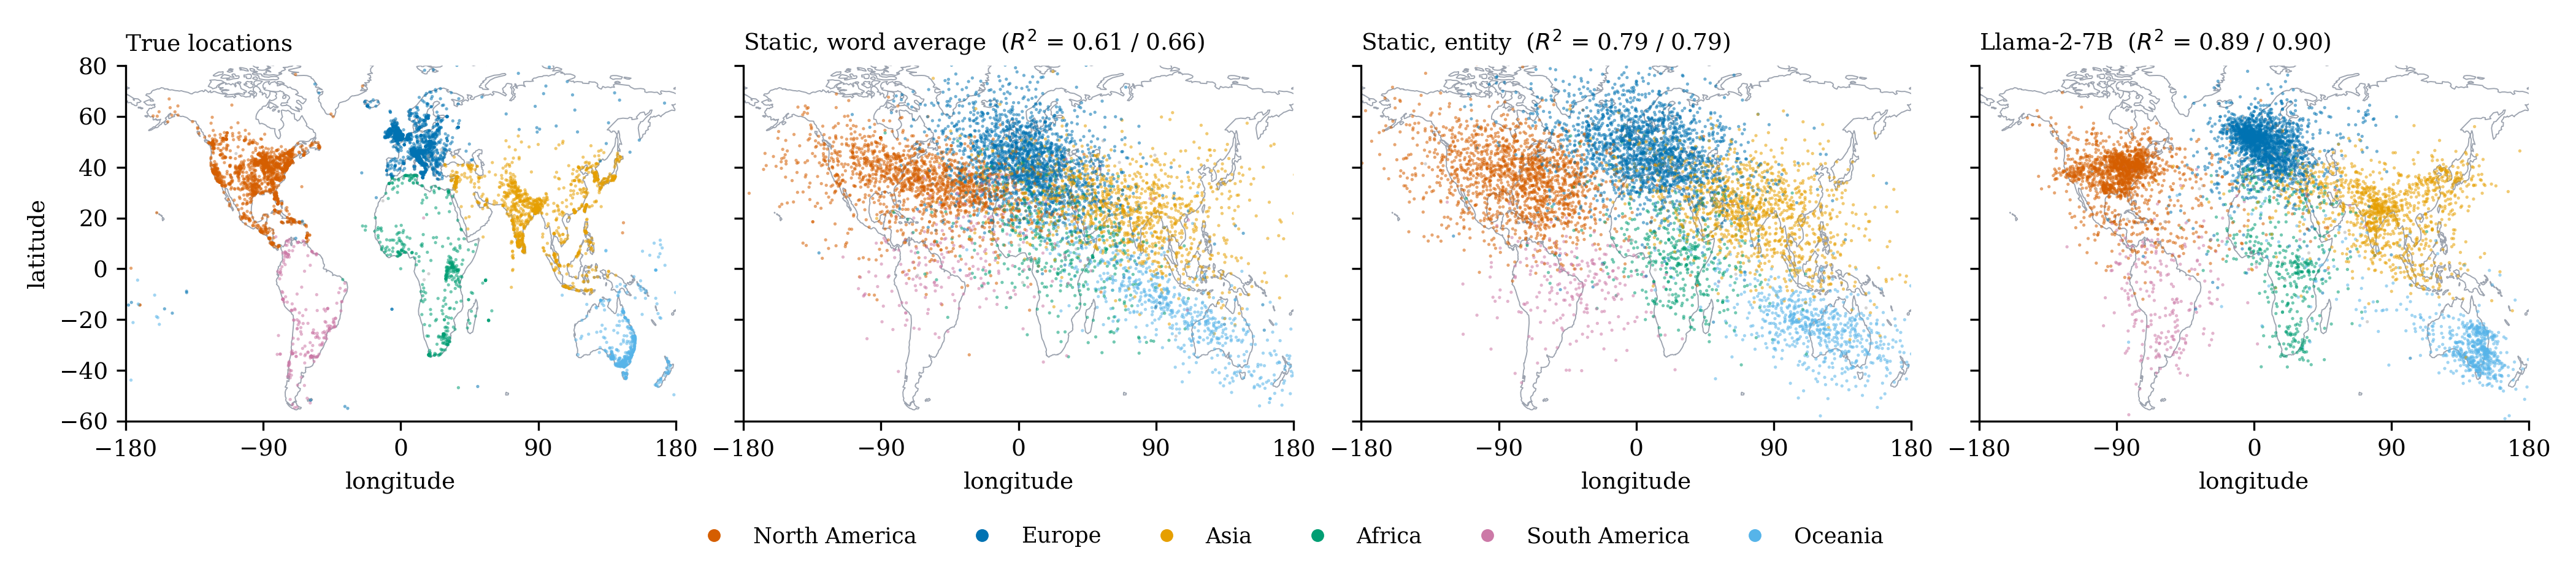
\includegraphics[width=\textwidth]{fig_entity_map_row.png}
  \caption{Held-out places from \citet{gurnee2024language} that have a Wikipedia2Vec entity vector
  ($n = 5{,}984$), at their true locations and as decoded by linear probes on Wikipedia2Vec's word
  vectors averaged over the name, on its static entity vectors, and on Llama-2-7B (layer 24), drawn
  over coastlines as in \citet{gurnee2024language}'s Figure~1 (which shows Llama-2-70B); color marks
  the true continent. The entity vectors recover a blurred
  version of the layout that Llama-2 recovers more precisely (median error 2{,}450\,km against
  760\,km; Table~\ref{tab:entity}).}
  \label{fig:entity_map}
\end{figure}

\begin{table}[t]
  \centering
  \caption{Word-level and entity-level static vectors against the transformers on the released
  entities that have a Wikipedia2Vec entity vector (authors' split; $n_{\text{test}} = 5{,}984$
  places and $4{,}707$ figures). Within-group $r$ is within country for places and within century
  for figures; the median error is in kilometers or years. Transformers at the selected layer.}
  \label{tab:entity}
  \footnotesize
  \setlength{\tabcolsep}{4pt}
  \begin{tabular}{lcccccc}
    \toprule
    & \multicolumn{3}{c}{Places} & \multicolumn{3}{c}{Figures} \\
    \cmidrule(lr){2-4} \cmidrule(lr){5-7}
    Representation & $R^2$ (lat / lon) & Within $r$ & Median error & $R^2$ & Within $r$ & Median error \\
    \midrule
    GloVe, word average          & .48 / .55 & .07 / .05 & 3{,}480 & .54 & .04 & 175 \\
    fastText, word average       & .59 / .62 & .12 / .08 & 3{,}038 & .62 & .07 & 160 \\
    Wikipedia2Vec, word average  & .61 / .66 & .13 / .09 & 2{,}879 & .65 & .07 & 150 \\
    Wikipedia2Vec, entity        & .79 / .79 & .25 / .11 & 2{,}448 & .80 & .14 & 109 \\
    \midrule
    Pythia-2.8B                  & .77 / .81 & .21 / .13 & 1{,}192 & .74 & .10 & 124 \\
    Llama-2-7B                   & .89 / .90 & .36 / .24 & 758     & .82 & .12 & 84 \\
    \bottomrule
  \end{tabular}
\end{table}

\subsection{What the Recovered Structure Consists Of}
\label{sec:mechanism-summary}

We fit a linear map from the static embeddings to the transformer activations on training
rows and probe the predicted part and the residual separately (Appendix~\ref{sec:residual}).
On the released entities the static-predictable part takes out a third or less of the
activation variance but most of the probe's performance: removing it lowers $R^2$ on latitude
and longitude from $0.76$ and $0.79$ to $0.20$--$0.29$ for Pythia-2.8B and from $0.88$ to
$0.27$--$0.39$ for Llama-2-7B, and on year of death from $0.70$ to $0.21$--$0.25$ and from
$0.78$ to $0.29$--$0.33$, depending on the static model. Removing the same share of variance
along random directions, or static vectors assigned to the wrong entities, leaves performance
almost unchanged.

Because both kinds of representation carry country and century identity, this cannot show
whether what they share goes beyond group membership. We therefore also removed from the
activations everything linearly predictable from a one-hot code of each item's country or
century. This takes out a fifth to a quarter of the activation variance for places and under
4\% for figures, but nearly all of the probe's performance ($R^2 \leq 0.01$ on every target
in both models). A probe trained on what remains still orders items within their group
(Llama-2: $r = 0.55$ and $0.53$ within countries for latitude and longitude, $0.13$ within
centuries; Pythia: $0.47$, $0.49$ and $0.09$). Removing in addition the static structure that
goes beyond group membership lowers these to $0.46$, $0.39$ and $0.03$ for Llama-2 (Pythia:
$0.37$, $0.34$ and $0.00$), against $0.54$, $0.52$ and $0.13$ (Pythia: $0.46$, $0.49$ and
$0.09$) after removing a random subspace of the same variance; for every target in both models
the 95\% interval for this difference excludes zero, and appending the static vectors to the
activations raises $R^2$ by at most $0.01$ (Table~\ref{tab:groupremoval}, Appendix~\ref{sec:group_methods}).
What the two kinds of representation share is thus mostly coarse group membership, plus part of the within-country ordering of places and the transformers' weak ordering of figures within centuries.

Finally, a random split tests generalization only to new items from familiar groups. When
whole groups are held out, no representation we tested generalizes well: with each continent
held out in turn, every representation predicts the held-out coordinates worse than their mean
($R^2$ from $-0.94$ to $-0.22$ for the word vectors and transformers and $-0.03$ and $-0.68$ for the entity vectors, against $0.48$--$0.89$ under random splits), and with each block of death
years held out $R^2$ is $-0.27$ for the entity vectors and $-0.16$ and $-0.11$ for Word2Vec and GloVe but $0.11$ and $0.19$ for
Pythia and Llama-2 (Table~\ref{tab:grouped_holdout}; the city set is in Appendix~\ref{sec:holdout}).

\subsection{World Cities: Which Words Carry the Signal}
\label{sec:cities}

Our city set adds targets the released datasets lack and lets us ask which words carry the signal. Table~\ref{tab:world_results} (appendix) gives probe $R^2$ for the six city targets. Longitude,
latitude and temperature are well predicted by both embeddings (GloVe and Word2Vec
$R^2 = 0.79$ and $0.84$, $0.76$ and $0.83$, and $0.67$ and $0.72$, respectively), and
so is GDP per capita ($0.75$ and $0.80$), which is a national variable and follows
the country structure of the embeddings (Appendix~\ref{sec:ablation}). Population is
intermediate ($0.50$--$0.52$). Elevation is recovered weakly and unstably ($0.21$ and
$0.33$, varying by more than $\pm 0.10$ across splits).

\begin{figure}[t]
  \centering
  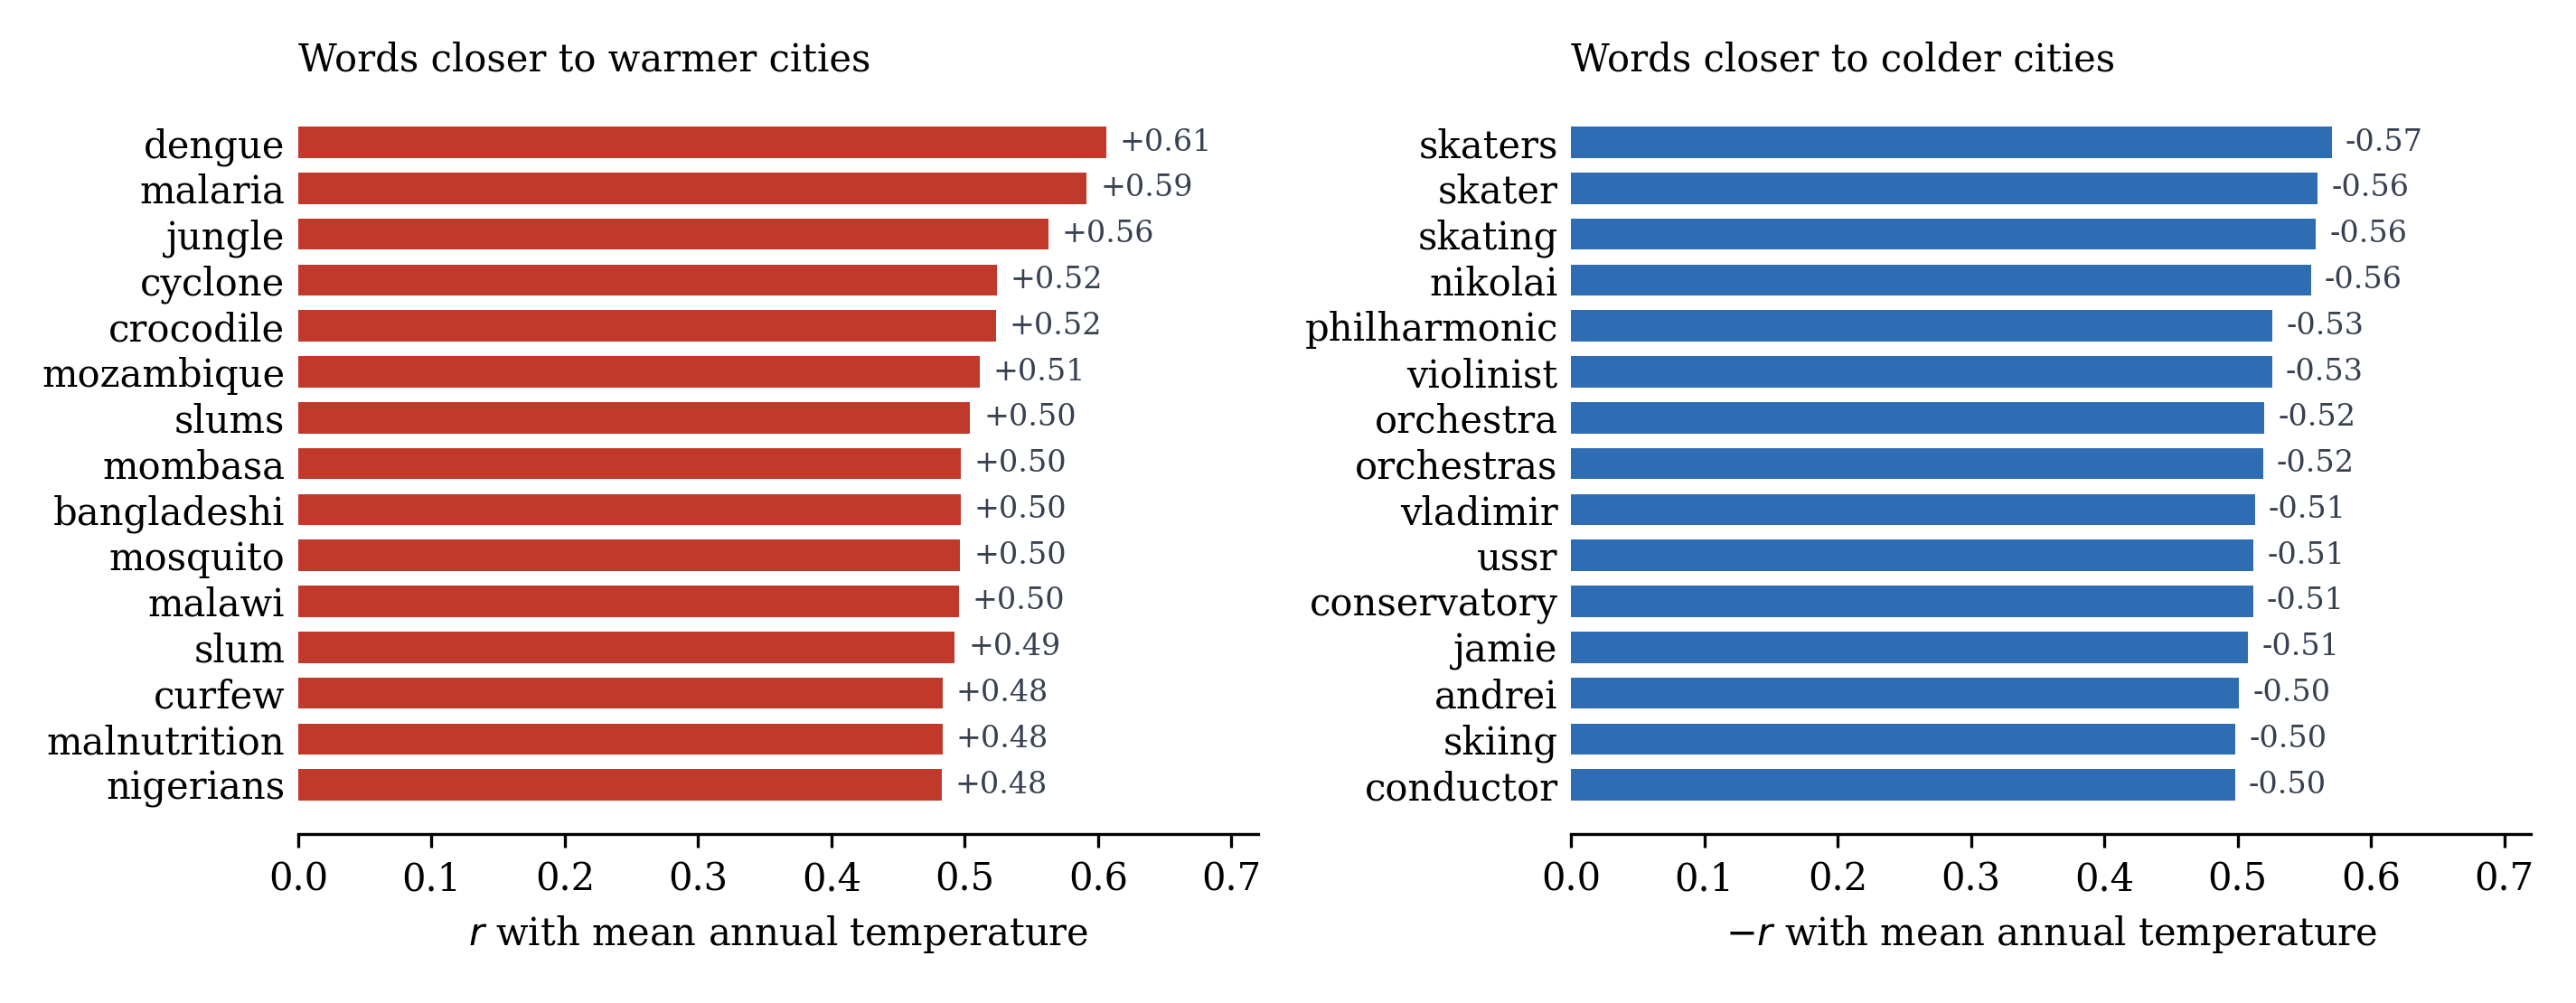
\includegraphics[width=0.62\textwidth]{fig_semantic_272_wide.png}
  \caption{Words whose GloVe vectors are closest to the names of warm and of cold cities. For each of 17{,}250 frequent words (the 20{,}000 most frequent GloVe words with at least four letters, excluding the cities' own name words and a list of common country names, demonyms and geographic terms), we correlate the word's cosine similarity to each of the 272 city names with the cities' mean annual temperature; shown are the 15 most positive and 15 most negative correlations. The words are selected for extreme correlations from the whole vocabulary, so the figure is descriptive and implies no significance.}
  \label{fig:semantic_spatial}
\end{figure}

This ordering of recoverability indicates to what extent each property is reflected in the
words a city's name appears with. Across our cities, the more similar a city name's representation is to those of \emph{malaria} or \emph{jungle},
the warmer the city tends to be, and the more similar it is to those of \emph{skiing} or
\emph{orchestra}, the colder it tends to be (Figure~\ref{fig:semantic_spatial}). Removing from the
embeddings the directions spanned by country names costs the probes more than removing any
other vocabulary, and, compared with matched random words, removing words for climate and
weather costs temperature most, latitude less and longitude nothing
(Appendix~\ref{sec:ablation}). The coordinates thus appear to be carried mainly by
associations with a city's country, the static counterpart of the coarse sorting we found in
the transformers (Section~\ref{sec:llm}), and temperature by associations with the
vocabulary of climate. No context-dependent computation over the city name is involved; the signal is already
available in a fixed lexical representation. Warm cities' names are close to \emph{malaria} and \emph{jungle}
not because temperature is explicitly represented as such, but because the names keep the same company as those words,
such as the names of tropical places (\emph{Borneo}, \emph{Cambodia}, \emph{Laos}); cold cities' names are close to \emph{skiing} and \emph{orchestra} through winter sports, Nordic places and Russian classical music (Appendix~\ref{sec:semantic}).
The probe finds the direction along which this shared company varies with temperature, and
thus seems to recover what text records about cities rather than a general store of facts
about them (see also Figure~\ref{fig:geography}).

\subsection{A ``Pain Axis''}
\label{sec:pain}

\citet{tagliabue2026pain} extract a ``pain direction'' from 25 open-weight models (2B to
72B parameters, five families). They report that it separates descriptions of painful
situations from matched controls, retains a component distinct from fear and negative valence
after their shared variance is removed, separates pain from injuries described as painless,
and, when added to the residual stream, produces first-person expressions of worthlessness
and failure. We reran their representational analyses with static word
embeddings (Section~\ref{sec:pain_methods}).

\begin{table}[t]
  \centering
  \caption{The pain-axis tests on static word embeddings, using the v2 stimuli of
  \citet{tagliabue2026pain}. Held-out AUC for pain against the S2 or S1
  controls and, for the S2 direction, the standalone Arousal and Random sets (mean $\pm$ s.d.\ over 20 fold assignments);
  $z$: mean projection of the standalone Numb and Sadness sets on the S2 direction,
  referenced to the S2 sentences (pain $\approx +0.7$, controls $\approx -0.7$). LLM values are the
  authors' held-out estimates; the keyword baseline is from \citet{painreview2026}.}
  \label{tab:pain}
  \small
  \begin{tabular}{lcccccc}
    \toprule
    & \multicolumn{4}{c}{Held-out AUC} & \multicolumn{2}{c}{$z$ on S2 direction} \\
    \cmidrule(lr){2-5} \cmidrule(lr){6-7}
    Representation & S2 & S1 & S2 vs.\ Arousal & S2 vs.\ Random & Numb & Sadness \\
    \midrule
    Keyword baseline & $0.727$ & $0.669$ & --- & --- & --- & --- \\
    GloVe    & $0.850 \pm 0.009$ & $0.773 \pm 0.011$ & $0.664$ & $0.815$ & $-0.07$ & $-0.09$ \\
    Word2Vec & $0.867 \pm 0.007$ & $0.802 \pm 0.012$ & $0.693$ & $0.857$ & $-0.38$ & $-0.48$ \\
    fastText & $0.878 \pm 0.006$ & $0.785 \pm 0.013$ & $0.712$ & $0.883$ & $-0.67$ & $-0.50$ \\
    \midrule
    25 LLMs  & $0.91$--$1.00$ & $0.85$--$0.94$ & all separate\textsuperscript{a} & all separate\textsuperscript{a} & $-0.4$--$+0.3$ & --- \\
    \bottomrule
    \multicolumn{7}{l}{\footnotesize \textsuperscript{a}Reported to separate pain from these sets in every model; values not given.}
  \end{tabular}

\end{table}

\paragraph{Separation.}
Averaged word vectors separate pain from controls on held-out sentence sets at AUC
$0.85$--$0.88$ on S2 and $0.77$--$0.80$ on S1 (Table~\ref{tab:pain}; see also
Figure~\ref{fig:pain} in the appendix). An independent review tested surface-lexical
baselines under the same
cross-validation, found at best $0.73$ and $0.67$, and concluded that the separation is not
lexical \citep{painreview2026}. That holds for surface features, but static embeddings
close about half the gap between keyword counts and the LLMs. The LLMs are still better on
held-out sets ($0.91$--$1.00$ on S2, $0.85$--$0.94$ on S1), even though their values come
from the best of many layers. The standalone sets show a clearer gap. The
static S2 direction separates held-out pain sentences from the Random set of everyday
statements (AUC $0.82$--$0.88$) but only weakly from the Arousal set of intense positive
experiences ($0.66$--$0.71$), and the S1 direction separates pain from neither
($0.44$--$0.60$), whereas the LLM directions separate pain from both in every model.

\paragraph{Specificity.}
The case that the direction encodes pain in particular, rather than distress in general,
originally rested on its low cosines with fear and negative emotion. In their second, more recent
version, the authors show that these values depend on how the directions are built: the pain
direction subtracts the pooled controls, which contain the fear and negative-emotion
sentences, so it is partly orthogonalized against them by construction. Built against a
common neutral baseline, the S2 direction's cosine with fear rises from $+0.12$ to $+0.58$
and with negative emotion from $+0.21$ to $+0.77$; built against the pooled controls, the
values are $+0.08$ and $+0.14$. We find that static embeddings reproduce this pattern under all three
constructions (Table~\ref{tab:pain_cos}, appendix). Both the large component that pain shares
with fear and negative emotion and the small residual that survives a common control
baseline are therefore present in averaged word vectors. The models differ in the residual
overlap with sadness, the largest the authors report ($+0.38$); in static embeddings it is
$+0.10$ to $+0.19$.

Injuries described as painless project well below the pain sentences ($z = -0.07$ to $-0.67$, against about $+0.7$), as in the models.

\paragraph{Summary.}
Averaged word vectors also separate pain from matched controls and show the same
construction-dependent overlap with fear and negative emotion. These tests reflect the
distributional structure of stimuli written to differ in exactly these ways and
do not by themselves show that the models represent pain. The models go further on held-out
separation, separation from arousal, the overlap with sadness and the vocabulary the direction
promotes (\emph{hurt}, \emph{shame}, \emph{worthless}); the
behavioral results lie outside what a representational baseline can test.

\subsection{Emotion Concepts: A Conceptual Replication}
\label{sec:emotion}

\citet{sofroniew2026emotion} report that emotion directions in Claude Sonnet 4.5 generalize
across contexts and causally influence the model's outputs (which they call \emph{functional
emotions}, without implying subjective experience). We test the representational claim that the
directions encode emotion concepts rather than emotion words, for which the evidence offered is
a prompt forbidding the story writer to use the emotion word or its synonyms
(Section~\ref{sec:emotion_methods}); since the original stories are not released, this tests
the protocol rather than Claude on the same stories. The prohibition removes the word but not the
vocabulary that goes with it. The authors' example for \emph{desperate} (their Appendix 6.6), a man facing arrest, out of a job and left by his wife, contains none of that word but many of the words found near it in text.

\paragraph{Results.}
On held-out topics, averaged word vectors separate each emotion from the other eleven at a
mean AUC of $0.84$--$0.88$, and assign stories to the right emotion 41--51\% of the time
(balanced accuracy, the mean recall over emotions, 44--54\%), against 8.3\% for a uniform
guess and 11.2\% for always choosing the most frequent held-out emotion (Table~\ref{tab:emotion}). The word directions, built from the
emotion labels alone, reach a mean AUC of $0.75$--$0.80$ and 12-way accuracy of 28--33\%
(balanced 29--35\%), three to four times chance. The story directions are reliably better than the word
directions (by $0.04$--$0.13$ in AUC and $0.06$--$0.28$ in accuracy, 95\% intervals over
held-out topics), but a substantial share of what they recover is already present in the
static vectors for the emotion words.

Because these stories were written to satisfy the prohibition, we also tested it on text
that was not. On GoEmotions, mean held-out AUC across the 27 emotions is $0.79$--$0.82$.
After removing every comment that contains an emotion word or a synonym, it is $0.78$--$0.81$,
a drop of about one point in each embedding. Most of the signal does not come from the
emotion words themselves.

\begin{table}[t]
  \centering
  \caption{Emotion directions on averaged static word vectors. Stories come from an
  independent replication corpus \citep{ogunlana2026qwenemotion} generated under the prompt
  of \citet{sofroniew2026emotion}; topics are held out, and brackets give 95\% intervals from
  resampling held-out topics. The word direction uses the emotion label's static vector and no
  stories. GoEmotions \citep{demszky2020goemotions} has 27 emotions in human-written text; the
  last column excludes every comment containing an emotion word or synonym.}
  \label{tab:emotion}
  \small
  \begin{tabular}{lccccc}
    \toprule
    & \multicolumn{2}{c}{Replication stories (12 emotions)} & & \multicolumn{2}{c}{GoEmotions (27 emotions)} \\
    \cmidrule(lr){2-3} \cmidrule(lr){5-6}
    & AUC & 12-way acc. & & all text & emotion words removed \\
    \midrule
    GloVe, story direction    & $0.838$ {\scriptsize [.82, .86]} & $0.415$ {\scriptsize [.36, .48]} & & $0.791$ & $0.783$ \\
    GloVe, word direction     & $0.752$ {\scriptsize [.72, .78]} & $0.277$ {\scriptsize [.24, .32]} & & --- & --- \\
    Word2Vec, story direction & $0.873$ {\scriptsize [.85, .89]} & $0.484$ {\scriptsize [.41, .55]} & & $0.804$ & $0.794$ \\
    Word2Vec, word direction  & $0.779$ {\scriptsize [.75, .81]} & $0.330$ {\scriptsize [.27, .39]} & & --- & --- \\
    fastText, story direction & $0.876$ {\scriptsize [.85, .90]} & $0.511$ {\scriptsize [.45, .57]} & & $0.818$ & $0.811$ \\
    fastText, word direction  & $0.802$ {\scriptsize [.77, .83]} & $0.314$ {\scriptsize [.24, .38]} & & --- & --- \\
    \midrule
    Chance                    & $0.500$ & $0.083$ & & $0.500$ & $0.500$ \\
       \bottomrule
  \end{tabular}
\end{table}

\paragraph{Summary.}
Averaged static word vectors reproduce the evidence that emotion concepts can be decoded, that
decoding generalizes to new topics, and that it survives a ban on naming the emotion, and the
vectors for the emotion words alone reproduce most of it. These tests reflect the vocabulary of
stimuli written to differ in exactly this respect and do not on their own show
that a model represents emotion concepts in a stronger sense than a lexicon does. The authors'
graded scenarios, in which one quantity varies while the wording stays
nearly constant, cannot be tested with averaged word vectors, and the steering results lie
outside what a representational baseline can address; these are where evidence about the model
itself is most likely to be found.

\section{Discussion}
\label{sec:discussion}

The case for emergent spatial and temporal world models has rested mainly on three observations: that probes recover real-world variables accurately, that accuracy rises across layers, and that it extends to entities held out from probe training. Static embeddings recover a large share of what has been decoded: averaged word vectors explain about half the variance in place coordinates and year of death on the released datasets, and static vectors for disambiguated entities reach $R^2 = 0.79$ and $0.80$, matching Pythia-2.8B on coordinates and Llama-2-7B on year of death. Held-out accuracy holds for static embeddings too, and when whole continents or periods are held out no representation we tested generalizes well (Section~\ref{sec:mechanism-summary}). High accuracy alone therefore cannot distinguish a representation of the world from the distributional associations in the training text.

Language models do better than this baseline. On the items that have an entity vector, Llama-2-7B reaches $R^2 = 0.89$ and $0.90$ on coordinates, against $0.79$ for entity vectors, and its median error is 758~km against 2{,}448~km (Table~\ref{tab:entity}). However, much of that advantage lies in sorting items into the right group, the right country or the right century. A predictor that knows only each item's group already captures nearly all of the variance ($R^2 = 0.96$--$1.00$), while within groups the language models' gain is modest (Table~\ref{tab:gt_pythia}). Group membership is also the kind of information word associations carry: places in the same country share a language, a currency, institutions and neighboring places, and people from the same century share events and vocabulary. Ordering items \emph{within} a group, or placing a country relative to a distant one, is what a map or a timeline should support, and that is where the advantage over the baseline is smallest. Part of the rise in accuracy across layers reflects the model assembling multi-token names, but averaging a name's input embeddings does not close the gap, so most of it comes from processing in context; the added accuracy is again mostly placement in the right country or century (Table~\ref{tab:gt_pythia}).

We are not claiming, on the basis of these results, that language models necessarily lack internal models of the world. The language models' advantage over the baseline could reflect a more sophisticated encoding of distributional associations alone, or something of a different kind, and our comparisons cannot fully separate the two. The entity baseline should not be read as a capacity-matched competitor to the transformer: it is given each entity's identity, which a transformer must infer from the name, and it is trained on Wikipedia, the source of the datasets. It is an existence proof: once the correct referent is supplied, fixed distributional associations attached to that entity suffice to reproduce most of the probe performance. Our claim is simply that the evidence offered so far, decoding accuracy and generalization to held-out entities, does not by itself distinguish a representation of the world from distributional associations.

The baseline suggests a simple criterion for future work. Any decoding result should be reported against static embeddings on the same items, and the advantage should be characterized in two ways: its size, and its kind, that is, whether it is a finer sorting of the same type that associations provide or a structure of a different type. Distinguishing these requires tests that set the property in question against the words used, for example items whose described location or date differs from what their names and neighbors would suggest, or groups held out of training entirely (Section~\ref{sec:mechanism-summary} and Appendix~\ref{sec:grouped_holdout}); causal and behavioral effects, which no representational baseline can address, are a further source of evidence. Without such tests, a probe result is consistent with both readings. The baseline is cheap, needs no access to the model, and can be applied to any study in this literature. It is also a reminder of how much the company a word keeps \citep{firth1957synopsis} records about where things are, when they happened, and how situations feel to the people who describe them.

\paragraph{Limitations.}
The largest transformer we tested is Llama-2-7B, and the
strongest claims concern much larger models, which may carry more than coarse sorting or generalize
better to held-out continents or periods; the baseline should be run against them. Our comparisons are representational, so they do not
address causal and behavioral evidence, such as steering or the Othello interventions \citep{li2023emergent}, or whether a model uses what a
decoder can read. The baseline itself is deliberately simple: averaging word vectors
ignores word order, so it likely understates what word relations alone can provide, and our
separation of what the transformers share with it is linear. Items with an entity vector are easier for every representation, language models included (Appendix~\ref{sec:coverage}), so absolute accuracy on the common subset overstates accuracy on the full release. The emotion case rests on a
replication corpus rather than the original stories, and the city set is small and was chosen by hand.

\paragraph{Broader impact.}
Decoding and related representational results are increasingly discussed in connection with model welfare and sentience \citep{keeling2024tradeoffs}. Our
results caution against treating decodability as evidence of internal states, but do not
show that models lack such states; we hope the baseline makes such discussions better calibrated rather than dismissive.

\paragraph{Reproducibility.}
Code, derived data and the result files behind every reported value are available
\ifanon in the supplementary material\else at \url{https://github.com/elanbarenholtz/static-embeddings-space-time}\fi,
including the sourced city table and \texttt{static\_baseline.py}, which runs the baseline
on any labeled stimulus set. The entity analyses use the 300-dimensional English Wikipedia2Vec vectors (April 2018 release), which the supplementary scripts filter to the items used.\ifanon\else{} An earlier version of this work fitted the ridge probe
without an intercept and used city attributes compiled without recorded sources, including
founding year; all results here fit an intercept and use the sourced attributes described in
Section~\ref{sec:data}, without founding year, and the qualitative pattern is unchanged.\fi

\bibliography{references}
\bibliographystyle{tmlr}

\appendix

\section{Supporting Analyses}
\label{sec:appendix}

The analyses in this appendix characterize \emph{why} the type-level baseline
recovers what it does, and report controls on the baseline itself. They support the
results in Section~\ref{sec:results} but are not required for the argument.

\subsection{Additional Methods}
\label{sec:extra_methods}

\paragraph{City attributes.} For six cities whose DBpedia coordinates were evidently wrong
(more than $0.2^\circ$ from Wikidata's) we use Wikidata's. Population is the most recent dated
value for the administrative unit Wikidata records, so its definition varies across cities;
three missing elevations are taken from the Copernicus GLO-90 elevation model. Mean annual
temperature is the mean of the twelve monthly mean temperatures in WorldClim 2.1 (1970--2000
normals at 2.5 arc-minutes) at each city's coordinates. GDP per capita is in current US dollars
(2023 or the latest available year), shared by all cities in a country, with Taiwan's from its
statistics office and North Korea's from the UN Statistics Division.

\paragraph{Activation extraction.} Activations were extracted in 16-bit precision and checked
against a separately computed CPU reference on 60 random names per model and dataset (cosine
similarity $> 0.999$).

\paragraph{Layer selection.} Single-layer results use a layer chosen without the test
data. On the released entities, the authors' training partition is split once into an
inner training set (80\%) and a validation set (20\%); each saved layer is probed on the
inner training set and scored on the validation set, and the layer with the best validation
$R^2$ (averaged over targets) is refitted on the full training partition and scored once on
the test partition. This selects layer~24 for Pythia-2.8B on places and layer~28 on
figures, and layer~24 for Llama-2-7B on both. On the city set the layer is chosen within
each of the ten outer splits by five-fold cross-validation on that split's training rows.
Analyses carried out at a single layer (residualization, error correlations, matched
dimensionality, neighbor availability) use, in each split, the layer selected for that split,
and their results are averaged over the ten test folds, so no held-out city influences the
layer used to evaluate it. For the grouped holdouts, where the authors' training partition
contains items from every continent and period, the transformer layer is instead fixed in
advance at layer~19 (60\% depth), so no held-out continent or period influences it either. In every case the ridge
penalty is chosen within the training rows by the same leave-one-out procedure, and principal
components are fitted on training rows only. Choosing the layer on the test data instead,
as in an earlier version of this analysis, changes the reported $R^2$ by at most $0.013$.

\paragraph{Pain directions.} The other
directions (fear, negative emotion, negative world state, bodily sensation, arousal, random,
numb, sadness) are each set's mean minus the mean of the neutral sentences, pooled over S1
and S2, and denoised against that neutral cloud. Following v2, we also rebuild every direction,
pain included, under two common baselines: against the pooled neutral sentences
(\emph{common neutral}) and against the pooled control sentences of S1 and S2
(\emph{common controls}), each denoised against its own cloud. Projections of the standalone
sets are $z$-scored against the S2 sentences and averaged over first- and third-person
versions. Removing the shared ``I feel:'' suffix changes no
value by more than $0.01$.

\paragraph{GoEmotions.} GoEmotions \citep{demszky2020goemotions} consists of Reddit comments labeled with 27 emotions or neutral, with its official train and test split (43{,}410 and
5{,}427 comments). Because comments can carry several labels, the positives for each emotion
are the comments with that label and the negatives all others. The direction is the mean of
the training positives minus the mean of the training negatives, denoised against comments
labeled only neutral, and we report the macro-average test AUC over the 27 emotions. For the
emotion-word control we remove every comment, in training and test, that contains one of the
27 label words, a WordNet synonym of one, or a derivationally related form (244 words in
all), which removes about a quarter of the comments.

\subsection{Residualizing the Transformer against the Type-Level Baseline}
\label{sec:residual_methods}

To test whether the transformer's recoverable structure is the static structure, we fit
a linear map from the $272 \times 300$ static embedding matrix $S$ to the
$272 \times d$ activation matrix $A$ at each layer, and decompose
$A = SB + (A - SB)$. We call $SB$ the \emph{projection} and $A - SB$ the
\emph{residual}, and probe each as we probe $A$ itself.

Three details matter. First, $B$ is estimated by ridge rather than least squares: a
random split leaves 217 training rows against 300 predictors, and an unregularized fit
would reproduce the training rows exactly, driving their residuals to zero and rigging
the outcome. The penalty is selected by cross-validation on the training rows. Second,
$B$ is refit inside every fold from that fold's training rows only, so no test city
influences its own reconstruction; the decomposition never touches the target, so this
is a conservative rather than a necessary choice. Third, because the projection is a
linear function of $S$, it contains no linearly available information beyond $S$;
separately regularized ridge fits can still differ slightly, because the transformation
changes the effective penalty. The projection serves as a consistency check on the fit, not
as a result.

Two nulls accompany the removal, because two distinct objections apply. The
\emph{variance-matched null} removes a random subspace of activation space, with its
dimension chosen so that the fraction of activation variance removed matches that of
the true removal; it answers whether a removal of this magnitude would have had this
effect regardless of what was removed. The \emph{shuffled-static null} repeats the true
removal with static vectors assigned to the wrong cities; it answers whether the effect
depends on the city correspondence or is an artifact of the regression.

We report two further tests that involve no removal. First, we correlate the signed
prediction errors of the transformer probe and the static probe within each test fold,
with the target partialed out---two weak probes both predict near the mean, so their
raw error vectors both approach $-(y - \bar{y})$ and correlate near unity for reasons
unrelated to any shared mechanism. Second, we correlate each city's absolute probe error with the
cosine similarity of its nearest training neighbors, with continent partialed out, in both
representation spaces, using one observation per city.

\subsection{Removing Group Membership from the Activations}
\label{sec:group_methods}

These analyses use the released entities, the authors' train--test split, the GloVe-covered
items and the training-selected layer of each model. Activations $A$ and static vectors $S$
are centered on training rows. Group membership $G$ is a one-hot code of country (places)
or century of death (figures); a group that occurs only in the test set gets a row of zeros.
Each removal fits a ridge map from a source matrix to a target matrix on training rows only,
with the penalty chosen on training rows by the same leave-one-out procedure, and subtracts the map's
prediction for every row, so no test item influences its own removal. \emph{Group removed}:
$R_G = A - \hat{A}(G)$, the activations minus their part predictable from group
membership. \emph{Group and static removed}: $S$ is first residualized on $G$ in the same
way, giving $S_\perp$, the static structure beyond group membership, and the part of $R_G$
predictable from $S_\perp$ is then removed. \emph{Group and random removed}: instead of the
$S_\perp$ component, a random subspace of $R_G$ (random orthonormal directions) is removed,
with as many directions as needed to remove the same share of $R_G$'s training-row variance.
For each condition a new probe is fitted on training rows and scored once on the test set;
within-group $r$ is computed after removing test-set country or century means from
predictions and targets. For the incremental analysis, $A$ and $S$ are each divided by
their mean training-row standard deviation and concatenated before probing. Intervals are
95\% percentile intervals over 1{,}000 resamples of test-set countries or centuries, with
the fitted probes held fixed. Table~\ref{tab:groupremoval} gives the full sequence.

\begin{table}[t]
  \centering
  \caption{Removing group membership from the activations (released entities, training-selected
  layers; Appendix~\ref{sec:group_methods}). $R^2$ for latitude / longitude and year of
  death, and within-country (places) or within-century (figures) $r$ of a probe refitted
  after each removal. The last row gives the within-group $r$ after removing the static
  component beyond group membership minus that after the matched random removal, with 95\%
  intervals from 1{,}000 resamples of test-set countries (273) or centuries (29).}
  \label{tab:groupremoval}
  \footnotesize
  \setlength{\tabcolsep}{4pt}
  \begin{tabular}{llcccc}
    \toprule
    & & \multicolumn{2}{c}{Places} & \multicolumn{2}{c}{Figures} \\
    \cmidrule(lr){3-4} \cmidrule(lr){5-6}
    Model & Condition & $R^2$ & Within-country $r$ & $R^2$ & Within-century $r$ \\
    \midrule
    Pythia-2.8B & Full activations             & .76 / .79 & .20 / .12 & .70 & .10 \\
                & Group removed                & .01 / .00 & .47 / .49 & .00 & .09 \\
                & Group + static removed       & .00 / .00 & .37 / .34 & .00 & .00 \\
                & Group + random removed       & .01 / .00 & .46 / .49 & .00 & .09 \\
                & Full + static appended       & .76 / .79 & .21 / .13 & .71 & .10 \\
                & Static $-$ random            & & $-.08$ [$-.12$, $-.02$] / $-.15$ [$-.19$, $-.04$] & & $-.09$ [$-.12$, $-.06$] \\
    \midrule
    Llama-2-7B  & Full activations             & .88 / .88 & .35 / .23 & .78 & .12 \\
                & Group removed                & .01 / .00 & .55 / .53 & .00 & .13 \\
                & Group + static removed       & .01 / .00 & .46 / .39 & .00 & .03 \\
                & Group + random removed       & .01 / .00 & .54 / .52 & .00 & .13 \\
                & Full + static appended       & .88 / .88 & .35 / .23 & .78 & .12 \\
                & Static $-$ random            & & $-.07$ [$-.13$, $-.03$] / $-.12$ [$-.17$, $-.04$] & & $-.10$ [$-.13$, $-.07$] \\
    \bottomrule
  \end{tabular}
\end{table}

\subsection{Grouped Holdouts on the Released Entities}
\label{sec:grouped_holdout}

For places, each item's continent is taken from its country (via the
\texttt{country\_converter} package) and the five main continents are used: Africa (2{,}406
GloVe-covered items), the Americas (9{,}953), Asia (7{,}104), Europe (9{,}614) and Oceania
(3{,}526); items whose country maps to no continent are left out. For figures, death year is
cut into five contiguous blocks of equal count: $-935$ to $1150$ ($n = 6{,}861$), $1151$--$1385$
($7{,}334$), $1386$--$1599$ ($7{,}426$), $1600$--$1814$ ($7{,}456$) and $1815$--$2021$
($7{,}507$). Each group is held out in turn, a probe is fitted on the remaining groups
(latitude and longitude jointly, as one multi-output ridge regression) and applied to the
held-out group, and $R^2$ is computed once over the pooled held-out predictions of all five
groups, each coordinate scored separately. For the transformers the layer is fixed in
advance at layer~19 (60\% depth, the depth used by \citet{gurnee2024language}) rather than
selected on the authors' training partition, which contains items from every continent and
period. $R^2$ within a single held-out group is not informative, because its denominator is
that group's small internal variance, so Table~\ref{tab:grouped_holdout} gives the median
absolute error for each held-out group. Predicting the earliest and latest blocks requires
extrapolation beyond the training range; the three middle blocks are periods surrounded by
training data, so predicting them is generalization across an unseen interval rather than
extrapolation.

\begin{table}[t]
  \centering
  \caption{Grouped holdouts on the released entities (transformers at the fixed layer~19). Median
  absolute error for each held-out group (degrees of latitude / longitude; years), the
  pooled $R^2$ over all held-out predictions, and, for comparison, $R^2$ and median error
  under random five-fold splits of the same items.}
  \label{tab:grouped_holdout}
  \footnotesize
  \setlength{\tabcolsep}{4pt}
  \begin{tabular}{lcccc}
    \toprule
    & GloVe & Word2Vec & Pythia-2.8B & Llama-2-7B \\
    \midrule
    \multicolumn{5}{l}{\emph{Places, continent held out (median error, lat.\ / long.)}} \\
    Africa        & 24.7 / 32.9 & 23.6 / 28.4 & 17.5 / 25.8 & 19.5 / 16.9 \\
    Americas      & 19.1 / 141.9 & 16.0 / 144.9 & 18.9 / 142.3 & 26.6 / 152.5 \\
    Asia          & 12.0 / 76.9 & 9.7 / 90.2 & 9.0 / 63.2 & 6.5 / 70.3 \\
    Europe        & 37.8 / 38.7 & 38.1 / 32.4 & 39.7 / 26.0 & 34.4 / 23.6 \\
    Oceania       & 61.2 / 168.2 & 59.6 / 176.1 & 45.4 / 181.0 & 54.4 / 147.8 \\
    Pooled $R^2$  & $-.52$ / $-.89$ & $-.40$ / $-.94$ & $-.31$ / $-.74$ & $-.22$ / $-.64$ \\
    Random split: $R^2$ (median error) & .48 / .55 (12 / 34) & .56 / .60 (11 / 30) & .75 / .79 (5 / 13) & .89 / .89 (3 / 8) \\
    \midrule
    \multicolumn{5}{l}{\emph{Figures, period held out (median error, years)}} \\
    $-935$--$1150$ & 644 & 647 & 538 & 509 \\
    $1151$--$1385$ & 174 & 204 & 191 & 133 \\
    $1386$--$1599$ & 156 & 138 & 137 & 108 \\
    $1600$--$1814$ & 183 & 210 & 133 & 97 \\
    $1815$--$2021$ & 398 & 413 & 328 & 337 \\
    Pooled $R^2$  & $-.11$ & $-.16$ & $.11$ & $.19$ \\
    Random split: $R^2$ (median error) & .50 (174) & .43 (191) & .68 (139) & .78 (101) \\
    \bottomrule
  \end{tabular}
\end{table}

\subsection{Items With and Without an Entity Vector}
\label{sec:coverage}

Entity vectors exist for 89\% of places and 63\% of figures, and the comparison in Table~\ref{tab:entity} uses only those items. To see whether they are easier, we trained each non-entity representation on all training items and scored it separately on held-out items with and without an entity vector (Table~\ref{tab:coverage}). Items without one are harder for every representation, the language models included, by $0.13$--$0.28$ in $R^2$; part of the difference for figures is mechanical, since the uncovered figures have a narrower range of death years (standard deviation 396 against 482 years). The drop is of similar size across representations, so the comparison between them on the common subset is not distorted, but absolute accuracy there is higher than on the full release.

\begin{table}[t]
  \centering
  \caption{$R^2$ on held-out items with and without a Wikipedia2Vec entity vector, for probes trained on all training items (authors' split, GloVe-covered items; transformers at the selected layer). Test items: 5{,}995 covered and 695 uncovered places, 4{,}710 covered and 2{,}606 uncovered figures. Counts differ slightly from Table~\ref{tab:entity}, which also requires a Wikipedia2Vec word vector.}
  \label{tab:coverage}
  \small
  \begin{tabular}{lcccc}
    \toprule
    & \multicolumn{2}{c}{Places (lat / lon)} & \multicolumn{2}{c}{Figures (year)} \\
    \cmidrule(lr){2-3} \cmidrule(lr){4-5}
    Representation & With entity vector & Without & With & Without \\
    \midrule
    GloVe, word average    & .48 / .55 & .34 / .28 & .53 & .40 \\
    fastText, word average & .59 / .62 & .43 / .34 & .61 & .47 \\
    Pythia-2.8B            & .77 / .81 & .59 / .57 & .73 & .60 \\
    Llama-2-7B             & .89 / .90 & .70 / .71 & .82 & .68 \\
    \bottomrule
  \end{tabular}
\end{table}

\subsection{Pairwise Similarity, Distance and Co-membership}
\label{sec:distance_methods}

For all $\binom{272}{2} = 36{,}856$ city pairs we compute embedding cosine similarity,
great-circle distance, and same-country and same-continent indicators, and regress
similarity on all three predictors jointly. Pairs are not independent, so significance
is assessed by permuting \emph{city} labels (10{,}000 draws) and recomputing the
statistic, never by an analytic test on pairs.

\subsection{Semantic Similarity Analysis}

To investigate whether the geographic signal is interpretable, we take a data-driven approach: for every word in the GloVe vocabulary (restricted to the 20,000 most frequent common English words, filtering out proper nouns, city and country names, demonyms, and words shorter than four characters), we compute its cosine similarity to each of the 272 city embeddings (one value per city) and correlate these similarity values with the cities' actual latitudes and temperatures. This identifies the words whose distributional profiles most systematically track geographic location, without any \textit{a priori} word selection.

We also construct \emph{composite scores} by taking the difference in cosine similarity to antonym pairs (e.g., similarity to ``cold'' minus similarity to ``warm'') and test whether these continuous gradients predict geographic targets.

\subsection{Semantic Subspace Ablation}
\label{sec:ablation_methods}

To ask which vocabularies span the directions the probes rely on, we perform subspace ablation experiments on GloVe embeddings.
For each of six semantic categories---cardinal directions (16 words), climate and weather (27 words), region and continent names (28 words), country names (68 words), economic terms (27 words), and cultural/language terms (31 words)---we:
\begin{enumerate}
  \item Collect GloVe vectors for all words in the category.
  \item Compute the principal subspace they span via PCA, retaining components that capture 90\% of the variance (capped at 20 dimensions).
  \item Project each city embedding onto this subspace and subtract the projection, zeroing out the embedding's component along those semantic directions.
  \item Re-run the ridge regression probe on the ablated embeddings and measure $R^2$ drop relative to the full-embedding baseline.
\end{enumerate}

Because ablation removes dimensions from the embedding, any observed $R^2$ drop could reflect generic information loss rather than removal of semantically specific content. Random orthonormal subspaces of the same dimensionality are a weak control, because random directions in the 300-dimensional space are nearly orthogonal to the region occupied by word vectors, so removing any set of real word vectors costs more. We therefore compare each category with 200 random \emph{word sets} drawn from the 50{,}000 most frequent GloVe words and matched to it word by word on frequency decile, proper-name status (whether the capitalized form is more frequent than the lowercase form in the GoogleNews vocabulary) and vector norm (the closest norm among 20 candidates from the same decile and status). Each random set's subspace is built in the same way and truncated to the category's dimensionality. We report the category's drop as a $z$-score against these matched sets, with an empirical one-sided $p$ (the smallest possible value is $1/201$), and record the share of the city embeddings' variance each subspace removes, since vocabularies whose directions align more closely with the city vectors are expected to cost more.

\subsection{Additional Results}

\begin{table}[t]
  \centering
  \caption{The type-level baseline on the entity datasets released by
  \citet{gurnee2024language}, using their designated train--test split and their
  metric (out-of-sample $R^2$; for places, the mean over the two coordinates, as in
  their evaluation code). LLM values are their reported figures for linear probes at
  60\% layer depth (their Table~2). Coverage is the share of entity names with at
  least one in-vocabulary token; each representation is scored on the test items it covers.}
  \label{tab:gt}
  \small
  \begin{tabular}{lccccc}
    \toprule
    & \multicolumn{3}{c}{World places ($n_{\text{test}} \approx 6{,}900$)} & \multicolumn{2}{c}{Historical figures ($n_{\text{test}} \approx 7{,}300$)} \\
    \cmidrule(lr){2-4} \cmidrule(lr){5-6}
    Representation & Latitude & Longitude & Both & Death year & Coverage \\
    \midrule
    GloVe            & $0.469$ & $0.526$ & $0.497$ & $0.496$ & 85\% / 98\% \\
    Word2Vec         & $0.547$ & $0.573$ & $0.560$ & $0.421$ & 88\% / 97\% \\
    fastText         & $0.586$ & $0.594$ & $0.590$ & $0.574$ & 92\% / 98\% \\
    \midrule
    Llama-2-7B       & ---     & ---     & $0.881$ & $0.785$ & --- \\
    Llama-2-13B      & ---     & ---     & $0.896$ & $0.804$ & --- \\
    Llama-2-70B      & ---     & ---     & $\mathbf{0.911}$ & $\mathbf{0.835}$ & --- \\
    \bottomrule
  \end{tabular}
\end{table}

\begin{figure}[t]
  \centering
  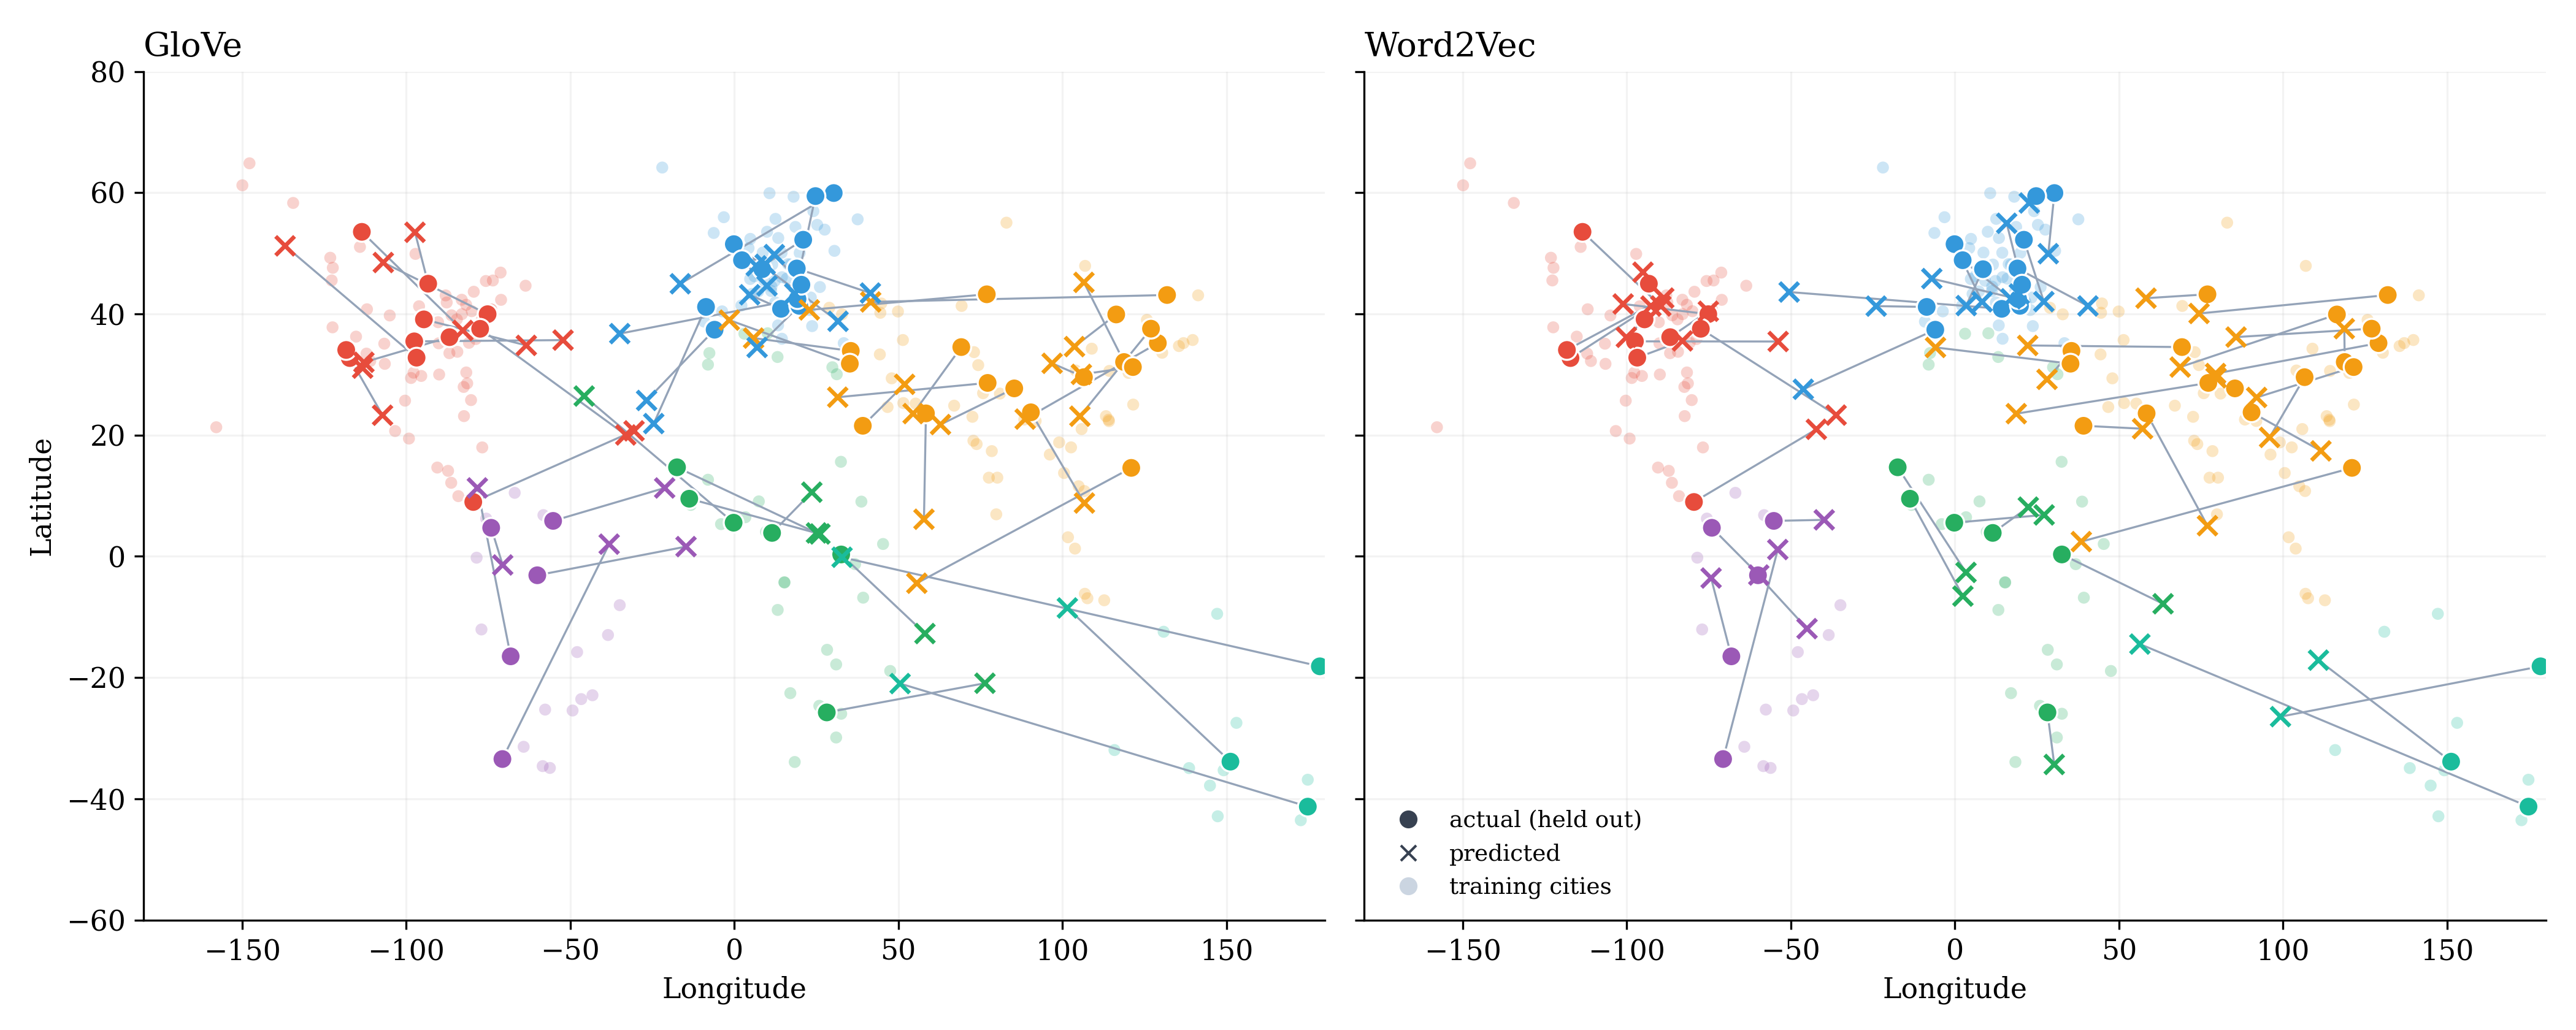
\includegraphics[width=\textwidth]{fig1_geography.png}
  \caption{Predicted city locations from ridge regression probes on GloVe (left) and Word2Vec (right) embeddings, for the held-out 20\% of 272 cities. Faded dots are training cities; filled circles are the true locations of held-out cities and crosses their predicted locations, joined by a line. Color denotes continent. Both models recover the broad continental layout from co-occurrence statistics alone.}
  \label{fig:geography}
\end{figure}

\begin{table}[t]
  \centering
  \caption{Pythia and static embeddings on the same 272 cities, under random 80/20 splits.
  Transformer values use a layer selected separately in each split by five-fold
  cross-validation on that split's training rows (Section~\ref{sec:llm_methods}), and
  within-continent $r$ is measured at that layer. Static values are Word2Vec, the better of the two static models
  on every measure. Layer~0 is the token-embedding output, before any attention. The
  continent one-hot carries only continent identity, so its within-continent $r$ is zero.}
  \label{tab:llm}
  \small
  \begin{tabular}{lcccccccc}
    \toprule
    & \multicolumn{5}{c}{$R^2$} & \multicolumn{3}{c}{Within-continent $r$} \\
    \cmidrule(lr){2-6} \cmidrule(lr){7-9}
    Target & 1.4B & 2.8B & 2.8B L0 & Static & Continent & 1.4B & 2.8B & Static \\
    \midrule
    Latitude    & $0.716$ & $0.800$ & $0.140$ & $0.833$ & $0.731$ & $0.670$ & $0.736$ & $0.755$ \\
    Longitude   & $0.764$ & $0.810$ & $0.325$ & $0.837$ & $0.915$ & $0.478$ & $0.475$ & $0.519$ \\
    Temperature & $0.686$ & $0.711$ & $0.158$ & $0.720$ & $0.290$ & $0.769$ & $0.790$ & $0.792$ \\
    \bottomrule
  \end{tabular}
\end{table}

\begin{table}[t]
  \centering
  \caption{Ridge regression probe $R^2$ for 272 world cities, mean $\pm$ s.d.\ over ten random 80/20 train/test splits. Geographic, climatic and national-economic targets are well recovered; elevation is recovered weakly and inconsistently.}
  \label{tab:world_results}
  \small
  \setlength{\tabcolsep}{4pt}
  \begin{tabular}{lcccccc}
    \toprule
    & Longitude & Latitude & Temperature & GDP per capita & Population & Elevation \\
    \midrule
    GloVe    & $0.788 \pm 0.039$ & $0.760 \pm 0.031$ & $0.675 \pm 0.061$ & $0.751 \pm 0.043$ & $0.500 \pm 0.100$ & $0.212 \pm 0.109$ \\
    Word2Vec & $0.837 \pm 0.035$ & $0.833 \pm 0.038$ & $0.720 \pm 0.038$ & $0.803 \pm 0.028$ & $0.515 \pm 0.066$ & $0.327 \pm 0.158$ \\
    \bottomrule
  \end{tabular}
\end{table}

\paragraph{Pythia on the city set.} In Pythia-2.8B, latitude goes from $R^2 = 0.140$ at
layer~0 to about $0.80$ by layer~20, and longitude from $0.325$ to about $0.81$ by
layer~27 (Figure~\ref{fig:llmlayers}); because 97\% of the names span several tokens, part
of this rise is the model assembling the name. With the layer selected within each training
split, Pythia-2.8B comes close to Word2Vec on temperature ($0.711$ against $0.720$) even
though it gives the probe 2560 features against 300. With both reduced to 200 principal
components (fitted on training rows), Pythia-2.8B reaches $0.794$, $0.808$ and $0.713$ at
the training-selected layers against GloVe's $0.759$, $0.788$ and $0.675$, so its edge over
GloVe is not only a matter of dimensionality. Within continents, correlating predictions
with targets after removing continent means gives $r = 0.67$--$0.74$ for latitude, $0.48$
for longitude and $0.77$--$0.79$ for temperature in the two Pythia models, against $0.76$, $0.52$ and $0.79$ for Word2Vec (Table~\ref{tab:llm}). A continent label predicts longitude
better than any of them ($R^2 = 0.92$) and latitude nearly as well ($0.73$), so most of what
every representation recovers on the coordinates is which continent a city is on.
Temperature is different: the continent label reaches only $0.29$, and most of what is
recovered lies within continents.

\begin{figure}[t]
  \centering
  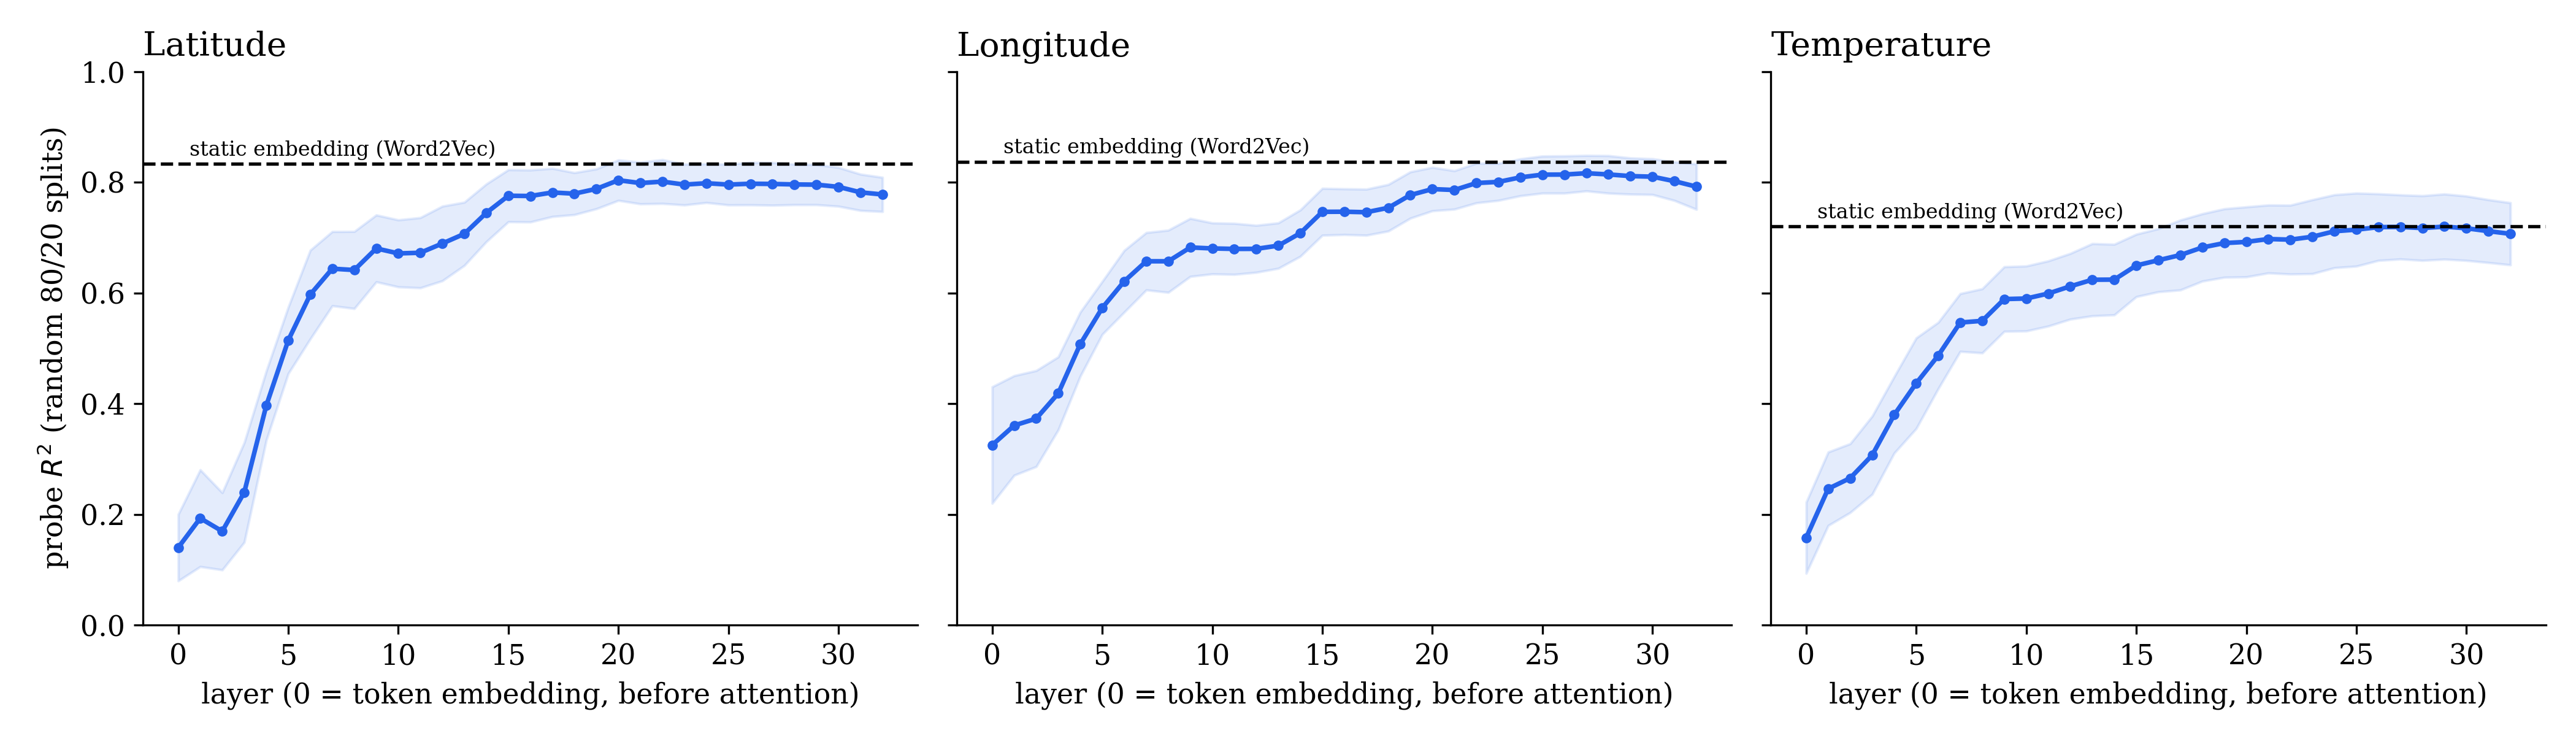
\includegraphics[width=\textwidth]{llm_layers_pythia-2.8b.png}
  \caption{Probe $R^2$ by layer for Pythia-2.8B on the 272-city dataset under random 80/20
  splits (shaded $\pm 1$ s.d.\ over ten splits). Layer~0 is the token-embedding output,
  before any attention; 97\% of these city names span several tokens, so layer~0 is the
  embedding of a final subword and the name has to be assembled by attention in later
  layers. The dashed line is the better static model (Word2Vec).}
  \label{fig:llmlayers}
\end{figure}

\begin{figure}[t]
  \centering
  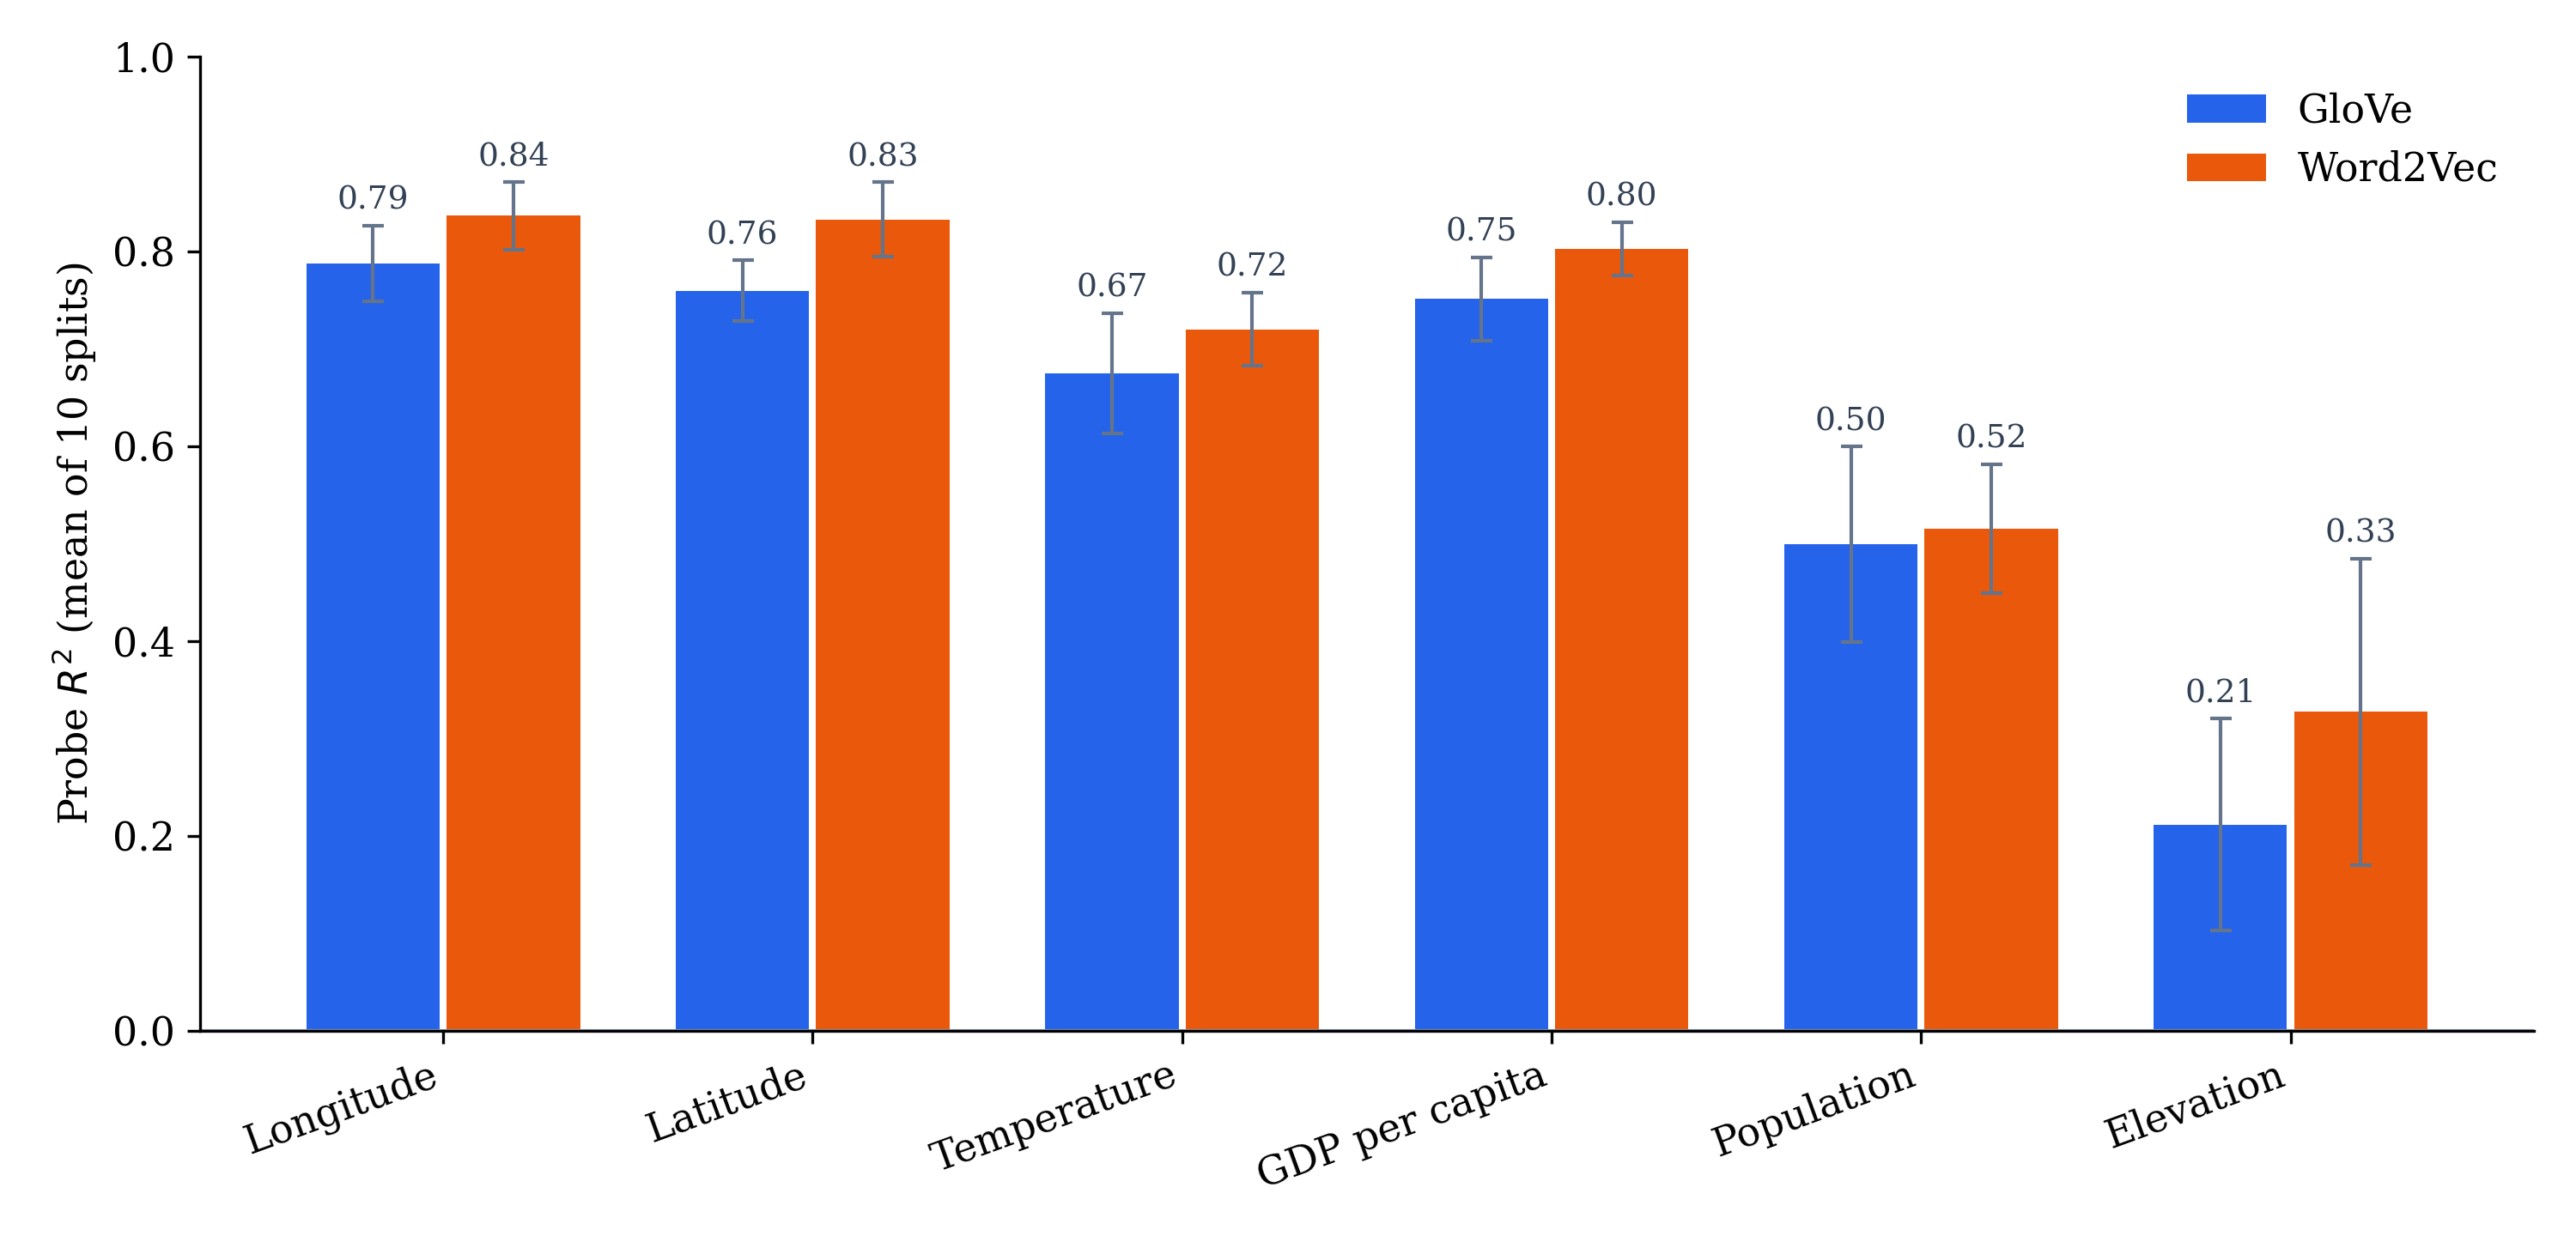
\includegraphics[width=0.85\textwidth]{fig2_barplot.png}
  \caption{Probe $R^2$ for all six city targets, comparing GloVe and Word2Vec. Bars show the mean over ten random 80/20 train/test splits; error bars show $\pm 1$ s.d. Geographic, climatic and national-economic targets yield high $R^2$; elevation is recovered weakly and with large variability across splits.}
  \label{fig:barplot}
\end{figure}

\begin{table}[t]
  \centering
  \caption{Cosine of the S2 pain direction with other directions on static word embeddings, under the original construction and the two common baselines of v2 \citep{tagliabue2026pain}. LLM values are the means reported in v2 (23--25 models).}
  \label{tab:pain_cos}
  \small
  \begin{tabular}{lccccccc}
    \toprule
    & \multicolumn{3}{c}{S2 $\times$ fear} & \multicolumn{3}{c}{S2 $\times$ negative emotion} & S2 $\times$ sadness \\
    \cmidrule(lr){2-4} \cmidrule(lr){5-7} \cmidrule(lr){8-8}
    Representation & Original & Neutral & Controls & Original & Neutral & Controls & Original \\
    \midrule
    GloVe    & $+0.05$ & $+0.61$ & $+0.11$ & $+0.23$ & $+0.76$ & $+0.08$ & $+0.19$ \\
    Word2Vec & $+0.03$ & $+0.54$ & $+0.13$ & $+0.19$ & $+0.71$ & $+0.10$ & $+0.10$ \\
    fastText & $-0.01$ & $+0.61$ & $+0.03$ & $+0.14$ & $+0.71$ & $+0.06$ & $+0.11$ \\
    \midrule
    LLMs (mean) & $+0.12$ & $+0.58$ & $+0.08$ & $+0.21$ & $+0.77$ & $+0.14$ & $+0.38$ \\
    \bottomrule
  \end{tabular}
\end{table}

\begin{figure}[t]
  \centering
  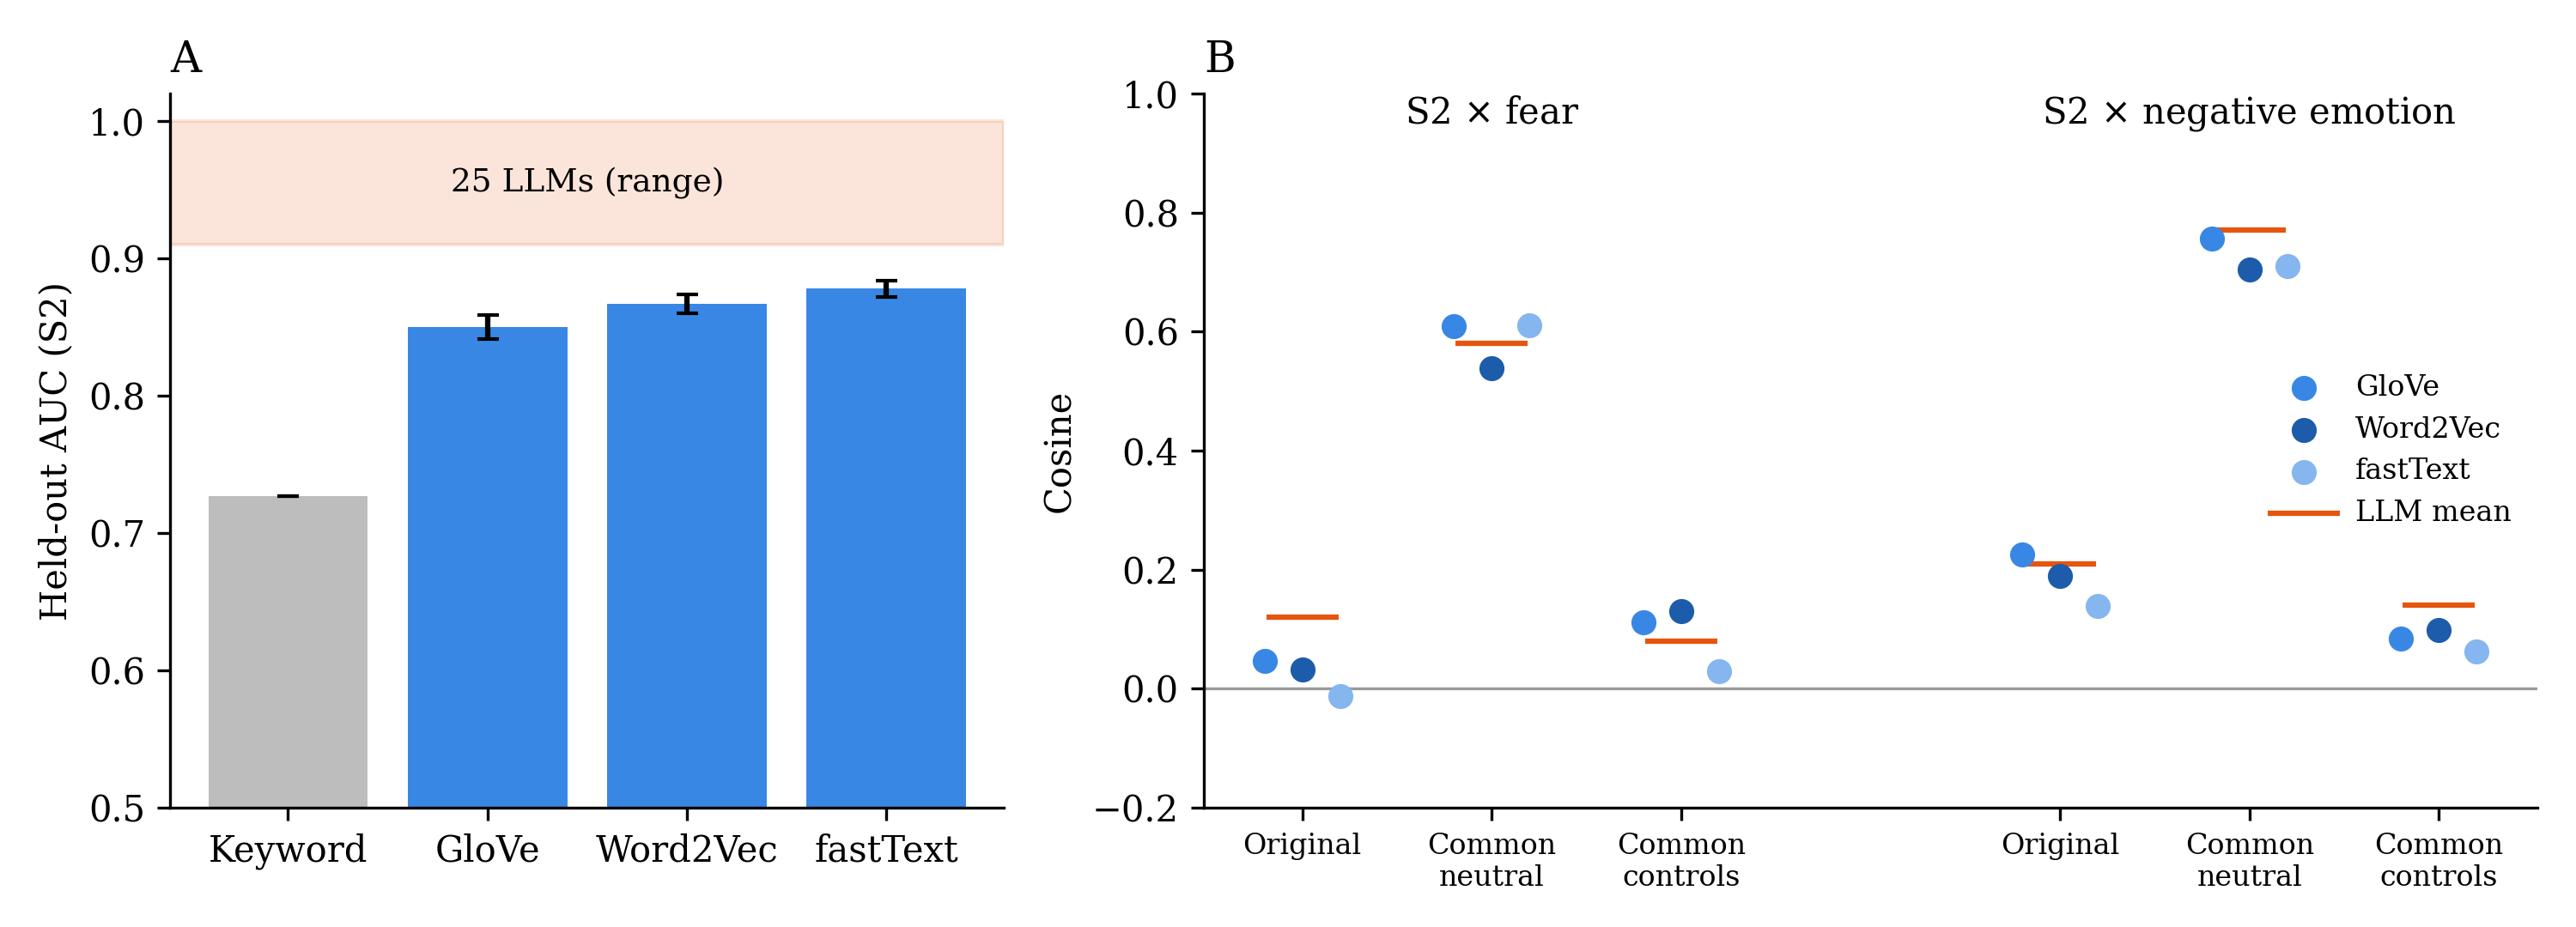
\includegraphics[width=\textwidth]{pain_static_baseline.png}
  \caption{The representational tests reported for a ``pain axis'' in 25 LLMs
  \citep{tagliabue2026pain}, run on averaged static word vectors of the authors' own
  sentences. \emph{A}: held-out separation of pain from controls (S2, first person;
  five-fold cross-validation over sentence sets, mean $\pm$ s.d.\ over 20 fold
  assignments). The keyword baseline is the best of several surface-lexical classifiers
  reported by an independent review \citep{painreview2026}. LLM values are each model's
  best layer. \emph{B}: cosine of the pain direction with fear, negative-emotion and
  negative-world-state directions; bars span the LLMs' per-model range.}
  \label{fig:pain}
\end{figure}

\subsection{Most Probe-Relevant Transformer Information Overlaps Linearly with Static Structure}
\label{sec:residual}

Matching performance is consistent with the two representations exploiting the same
structure, but does not establish it. We test how far the probe-relevant information in the
activations overlaps linearly with the static embeddings. Overlap is not identity: if both
representations track the same coarse groupings, such as country or continent, a linear map
will find shared target-relevant variance even if the two arise differently (we test this
on the released entities in Section~\ref{sec:mechanism-summary}).

For each layer we fit a linear map from the 300-dimensional static vector of a city to
its 2560-dimensional activation, using training rows only, and split the activations
into the part that map predicts (the \emph{projection}) and what it misses (the
\emph{residual}). Both are then probed exactly as the full activations were. The
decomposition never sees latitude, longitude or temperature: it is fit entirely from
the correspondence between two representations of the same city, and is therefore
target-blind.

\begin{table}[t]
  \centering
  \caption{Removing the static-predictable component of Pythia-2.8B activations, in each
  split at the layer selected by cross-validation on that split's training rows
  (Section~\ref{sec:llm_methods}); values are means over the ten test folds. \emph{Var.\ removed} is the fraction of activation
  variance the removal takes out; the variance-matched null removes the same fraction
  along random, city-blind directions. The shuffled-static null repeats the removal
  with static vectors attached to the wrong cities.}
  \label{tab:residual}
  \small
  \begin{tabular}{llccccc}
    \toprule
    Target & Static removed & full & projection & \textbf{residual} & var.-matched null & var.\ removed \\
    \midrule
    Latitude    & GloVe    & $0.800$ & $0.763$ & $\mathbf{0.233}$ & $0.791$ & 34\% \\
    Longitude   & GloVe    & $0.810$ & $0.792$ & $\mathbf{0.128}$ & $0.810$ & 35\% \\
    Temperature & GloVe    & $0.711$ & $0.684$ & $\mathbf{0.220}$ & $0.711$ & 35\% \\
    \midrule
    Latitude    & Word2Vec & $0.800$ & $0.837$ & $\mathbf{0.172}$ & $0.789$ & 25\% \\
    Longitude   & Word2Vec & $0.810$ & $0.833$ & $\mathbf{0.129}$ & $0.809$ & 28\% \\
    Temperature & Word2Vec & $0.711$ & $0.733$ & $\mathbf{0.280}$ & $0.706$ & 26\% \\
    \bottomrule
  \end{tabular}
\end{table}

Table~\ref{tab:residual} and Figure~\ref{fig:residual} give the result. Removing the
static-predictable component reduces latitude recovery from $0.800$ to $0.233$
(GloVe) or $0.172$ (Word2Vec), longitude from $0.810$ to $0.128$--$0.129$, and temperature
from $0.711$ to $0.220$--$0.280$. Averaged over the plateau (layers 10--32) the residual
retains 16--34\% of the full value. The same analysis at 1.4B replicates: full values of
$0.716$, $0.764$ and $0.686$ fall to residuals of $0.213$, $0.205$ and $0.330$ against
GloVe and $0.179$, $0.255$ and $0.326$ against Word2Vec, retaining 25--48\%, with the
variance-matched null again leaving performance untouched ($0.710$, $0.765$, $0.678$).

Two controls establish that this is not an artifact of the amount removed. The
\emph{variance-matched null} deletes the same fraction of activation variance
(25--35\%) along random directions that carry no information about which city is which,
and leaves performance essentially untouched ($0.791$, $0.810$, $0.711$ against GloVe's
removal). The
\emph{shuffled-static null}, which repeats the removal with static vectors assigned to
the wrong cities, removes almost no variance and returns the full value exactly,
confirming that the removal depends on the city correspondence rather than on the
regression itself. What matters is not how much variance is removed but which.

The complementary condition is a consistency check rather than a finding: because the
projection is a linear function of the static vectors, it contains no additional linearly
available information. Separately regularized ridge fits can nevertheless differ slightly,
because the transformation changes the effective penalty; empirically the two values are
nearly identical ($0.763$ against GloVe's own $0.760$ for latitude; $0.837$
against Word2Vec's $0.833$).

\begin{figure}[t]
  \centering
  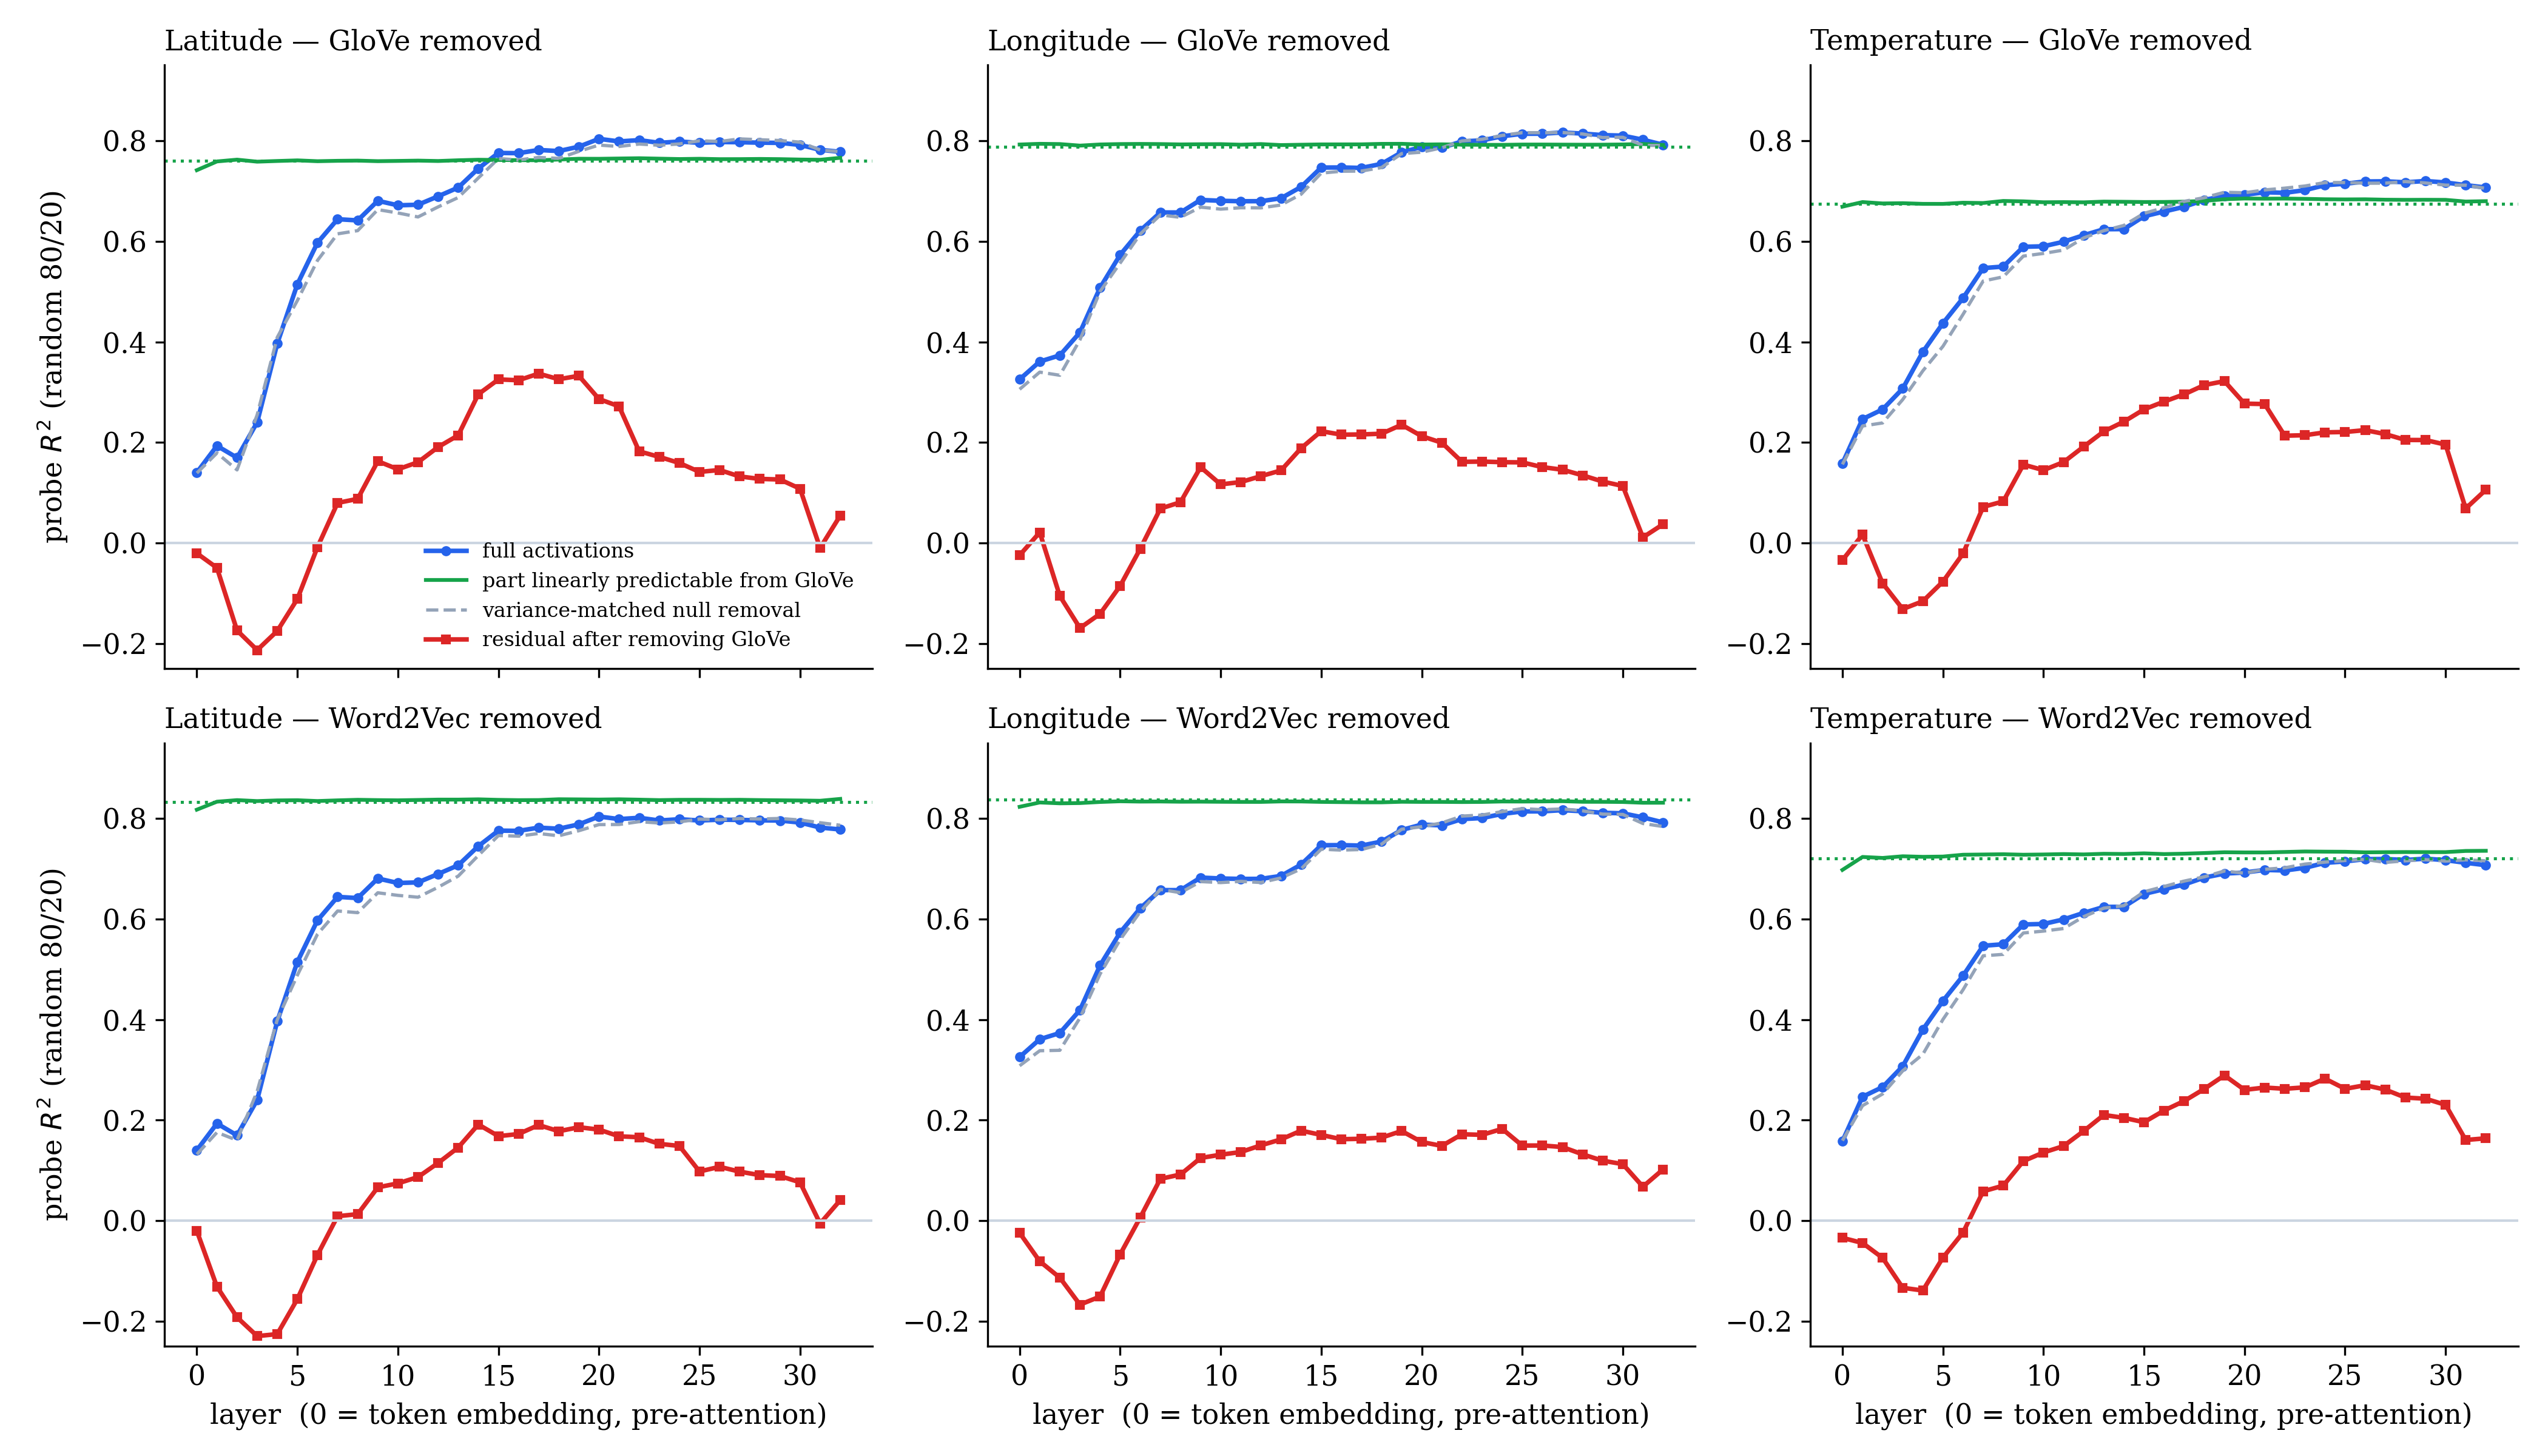
\includegraphics[width=\textwidth]{residualise_pythia-2.8b.png}
  \caption{Pythia-2.8B by layer: full activations (blue), the component linearly
  predictable from the static embedding (green), the residual after that component is
  removed (red), and a removal of matched variance along random directions (gray
  dashed). The dotted line is the static embedding probed directly. Most probe-relevant
  performance lies in the activation component linearly predictable from static embeddings,
  while a nonzero residual remains; removing matched variance along random directions has
  little effect.}
  \label{fig:residual}
\end{figure}

\paragraph{The two probes fail on the same cities.}
Signed prediction errors from the transformer probe and the static probe, correlated
within each test fold with the target partialed out, give $r = 0.41$--$0.58$ across
targets and static models, and $r = 0.27$--$0.44$ when computed within continent.
The floor for this measure---the transformer probe against a probe on matched random
features---is $-0.02$ to $0.08$. For calibration, the same measure applied to GloVe against
Word2Vec, two representations that share a distributional basis, gives $r = 0.52$--$0.62$.

\paragraph{Both show a modest relationship with neighbor availability.}
Probe error tends to rise as a city's nearest training neighbors become less similar, in
the static embeddings and, more weakly, in activation space. Each of the 239 cities that
fall in at least one test set contributes one observation: its absolute error and the mean
similarity of its five nearest training neighbors, each averaged over the splits in which it
was tested, with continent partialed out. The correlation is $r = -0.16$ (latitude,
$p = .01$), $-0.15$ ($p = .03$) and $-0.05$ ($p = .43$) in Pythia-2.8B activations,
against $-0.14$ ($p = .03$), $-0.27$ ($p < .001$) and $-0.19$ ($p = .004$) in GloVe. The
probes appear to answer partly by proximity to cities they were trained on, more clearly in
GloVe.

\subsection{What Carries the Recoverable Structure}
\label{sec:holdout}

Three analyses under the random 80/20 protocol ask how much of the recoverable structure
is coarse group membership, and a fourth asks how well items are ordered within their
group.

\paragraph{Six indicators outperform 300 dimensions.}
Replacing the embeddings with a six-element one-hot vector encoding continent membership
and nothing else (Table~\ref{tab:holdout}) recovers longitude at $R^2 = 0.915$, above
GloVe's $0.788$ and Word2Vec's $0.837$, and latitude at $0.731$, close to GloVe's
$0.760$. Temperature is the exception: continent identity alone yields only $0.290$
against GloVe's $0.675$.

\paragraph{Recoverability tracks between-group variance.}
The share of each target's variance that lies between continents ($\eta^2$) is $0.926$
for longitude, $0.747$ for latitude, $0.606$ for GDP per capita, $0.352$ for population,
$0.327$ for temperature and $0.109$ for elevation. Across the six targets, random-split
$R^2$ tracks $\eta^2$ at Pearson $r = 0.85$ and $0.87$ for GloVe and Word2Vec (Spearman
$0.94$ for both); excluding temperature, $r = 0.94$ and $0.95$. Temperature is the
residual, exceeding its $\eta^2$-predicted value by $+0.232$ (GloVe) and $+0.207$
(Word2Vec).

This is a fact about the targets and the sample, not only about the representations: a
variable whose variance is overwhelmingly between coarse groups can be recovered at
high $R^2$ by anything that identifies the group, without any finer-grained
information being present.

\paragraph{Decomposition.}
Substituting each city's vector with its continent's centroid (computed from training
rows only) and, separately, with its within-continent residual isolates the two
components under the random protocol.
For GloVe, latitude decomposes as $0.760$ (full), $0.731$ (centroid only), $+0.011$
(residual); longitude as $0.788$, $0.915$, $-0.018$; temperature as $0.675$, $0.287$,
$+0.242$. Word2Vec gives $0.833 / 0.731 / +0.002$, $0.837 / 0.915 / -0.021$ and
$0.720 / 0.288 / +0.315$. For the coordinates the centroid accounts for nearly all of the full $R^2$; for
temperature it accounts for less than half.

\paragraph{Holding out continents.}
Training on five continents and predicting the sixth, with predictions pooled over the six
held-out continents, GloVe and Word2Vec reach $R^2 = 0.003$ and $0.319$ for latitude,
$-0.246$ and $-0.218$ for longitude, and $0.476$ and $0.465$ for temperature, against
$0.76$--$0.83$, $0.79$--$0.84$ and $0.67$--$0.72$ under random splits. Random-split coordinate performance depends heavily on continent-specific
calibration, and the learned linear map transfers poorly to a continent it has not seen;
temperature, much of whose variance lies within continents, transfers substantially better.

\begin{table}[t]
  \centering
  \caption{Probe $R^2$ and within-continent ordering for the 272 cities under random 80/20
  splits (mean over ten splits). Within-continent $r$ correlates predictions with targets
  after removing continent means in each test set. The one-hot rows carry only country or
  continent identity (132 countries).}
  \label{tab:holdout}
  \small
  \begin{tabular}{llcc}
    \toprule
    Representation & Target & $R^2$ & Within-continent $r$ \\
    \midrule
    GloVe    & Latitude    & $0.760$ & $0.670$ \\
             & Longitude   & $0.788$ & $0.410$ \\
             & Temperature & $0.675$ & $0.743$ \\
    \midrule
    Word2Vec & Latitude    & $0.833$ & $0.755$ \\
             & Longitude   & $0.837$ & $0.519$ \\
             & Temperature & $0.720$ & $0.792$ \\
    \midrule
    Country one-hot   & Latitude    & $0.510$ & --- \\
                      & Longitude   & $0.754$ & --- \\
                      & Temperature & $0.364$ & --- \\
    \midrule
    Continent one-hot & Latitude    & $0.731$ & $0$ \\
                      & Longitude   & $0.915$ & $0$ \\
                      & Temperature & $0.290$ & $0$ \\
    \bottomrule
  \end{tabular}
\end{table}

\paragraph{Within-group ordering.}
Correlating predictions with targets after removing continent means measures ordering
inside continents alone, and a representation carrying only continent identity scores
zero. Under random splits GloVe orders cities within continents at $r = 0.67$ for
latitude, $0.41$ for longitude and $0.74$ for temperature, and Word2Vec at $0.76$, $0.52$
and $0.79$. The embeddings therefore carry position within continents as well as continent
identity, consistent with the dependence of similarity on distance
(Appendix~\ref{sec:distance}). The decomposition above does not show this, because a probe
trained on within-continent residuals is scored against the full target, most of whose
variance lies between continents.

\paragraph{Historical figures.}
On the released figures, year of death varies almost entirely between centuries
($\eta^2 = 0.996$ in the test set) and mostly between three eras (before 500\,CE,
500--1400, after 1400; $\eta^2 = 0.80$). As oracle decompositions derived from the target itself, an
era label accounts for $R^2 = 0.80$ and a century label for $1.00$, against $0.50$ for GloVe. Replacing each figure's GloVe vector
with its era's training centroid gives $0.80$, and the within-era residual gives $0.04$.
Within centuries, GloVe and Word2Vec order figures at $r = 0.05$.

\paragraph{Other targets.}
Across all six city properties, random-split $R^2$ tracks $\eta^2$. Elevation departs in
the other direction: it is recovered worst under the random split, yet its recovery is
least attributable to continent membership, with 63--82\% of its modest recoverability
surviving the removal of continent centroids, against 12--17\% for GDP. Recoverability and
group dependence are dissociable, so a high random-split $R^2$ does not by itself say what
kind of information a representation carries.

\subsection{Similarity Tracks Distance, Not Only Co-membership}
\label{sec:distance}

A natural reading of the preceding results is that embedding similarity is driven by
shared administrative and linguistic context rather than by geography as such. That is not
the whole explanation. Across all 36{,}856 city pairs, cosine similarity falls with great-circle distance
independently of co-membership. With log distance, same-country and same-continent
indicators entered together, the standardized coefficient on distance is $-0.375$
(GloVe) and $-0.409$ (Word2Vec), against $+0.134$ and $+0.082$ for same-country
membership. Distance continues to predict within every stratum: among same-country
pairs $r = -0.480$ and $-0.488$; among same-continent, different-country pairs $-0.388$
and $-0.353$; among pairs on different continents $-0.241$ and $-0.294$. Permuting city
labels (10{,}000 draws) puts the partial distance coefficient far outside its null
($-0.375$ against $0.000 \pm 0.020$, $p < .001$). Pairs under 500\,km apart in
\emph{different} countries are more similar (GloVe $0.419$, Word2Vec $0.503$) than
pairs over 2000\,km apart within the \emph{same} country ($0.293$, $0.364$).

The representations therefore carry genuine local metric structure.

\subsection{Dimensionality Scaling}
\label{sec:dimensionality}

To test whether the geographic signal scales smoothly with embedding capacity, we run ridge regression probes predicting latitude, longitude, and temperature from GloVe embeddings at four dimensionalities (50, 100, 200, 300) using the 272-city dataset, under the protocol of Table~\ref{tab:world_results} (mean over the same ten random 80/20 splits).

Figure~\ref{fig:dimscaling} shows that $R^2$ rises with dimensionality for all three targets, though longitude changes little beyond 100 dimensions and temperature beyond 200. Latitude $R^2$ rises from 0.53 (50d) to 0.76 (300d); longitude from 0.70 to 0.79; temperature from 0.53 to 0.67, with the 300d values matching Table~\ref{tab:world_results}. (An earlier version of this figure used a single split, which overstated temperature at 300d.) These results show an association between dimensionality and performance within the tested GloVe models. They do not establish how performance would scale beyond 300 dimensions, nor do they isolate dimensionality from the other differences between static embeddings and transformers---corpus size, contextual disambiguation, training objective and architecture all remain possible contributors. The dimension-matched comparison with Pythia in Appendix~\ref{sec:appendix} addresses this more directly, by holding the number of features constant across representations.

\begin{figure}[t]
  \centering
  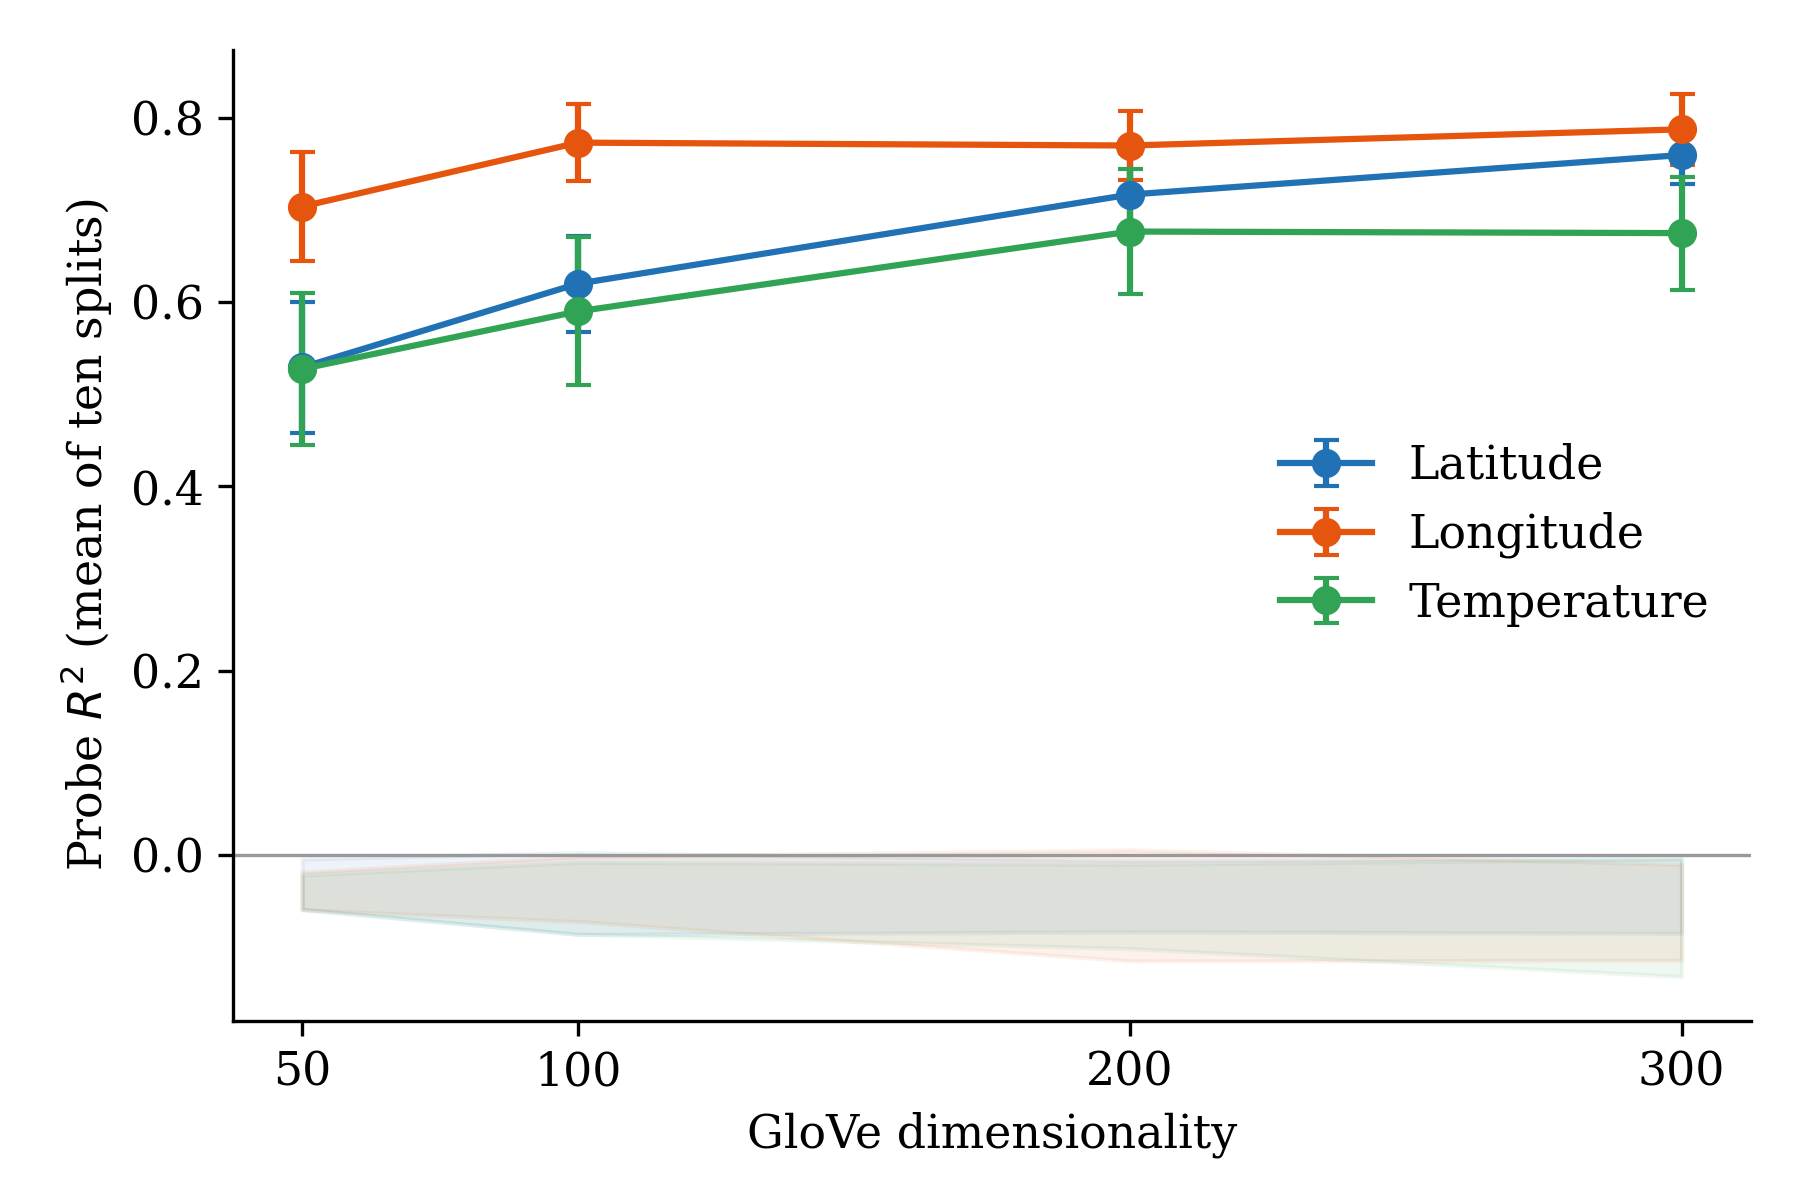
\includegraphics[width=0.65\textwidth]{fig_dimensionality_scaling.png}
  \caption{Probe $R^2$ versus GloVe embedding dimensionality for latitude, longitude, and temperature (272 cities). Points are means over the ten splits of Table~\ref{tab:world_results}, with error bars of $\pm 1$ s.d.; shaded bands show $\pm 2$ s.d.\ of matched random embedding baselines.}
  \label{fig:dimscaling}
\end{figure}

\subsection{Random Embedding Control}

To confirm that the probes do not find spurious structure in arbitrary high-dimensional vectors, we generate 20 sets of random Gaussian embeddings at each dimensionality (50, 100, 200, 300) and run the same probes over the same ten splits. Figure~\ref{fig:randomcontrol} shows that random embeddings yield $R^2 \approx 0$ (slightly negative) at all dimensionalities: arbitrary vectors of the same dimensionality do not reproduce the observed performance, so the structure recovered from GloVe is not an artifact of high-dimensional geometry or of the fitting procedure. This control does not address effects of entity selection, regional clustering among the sampled cities, or preprocessing.

\begin{figure}[t]
  \centering
  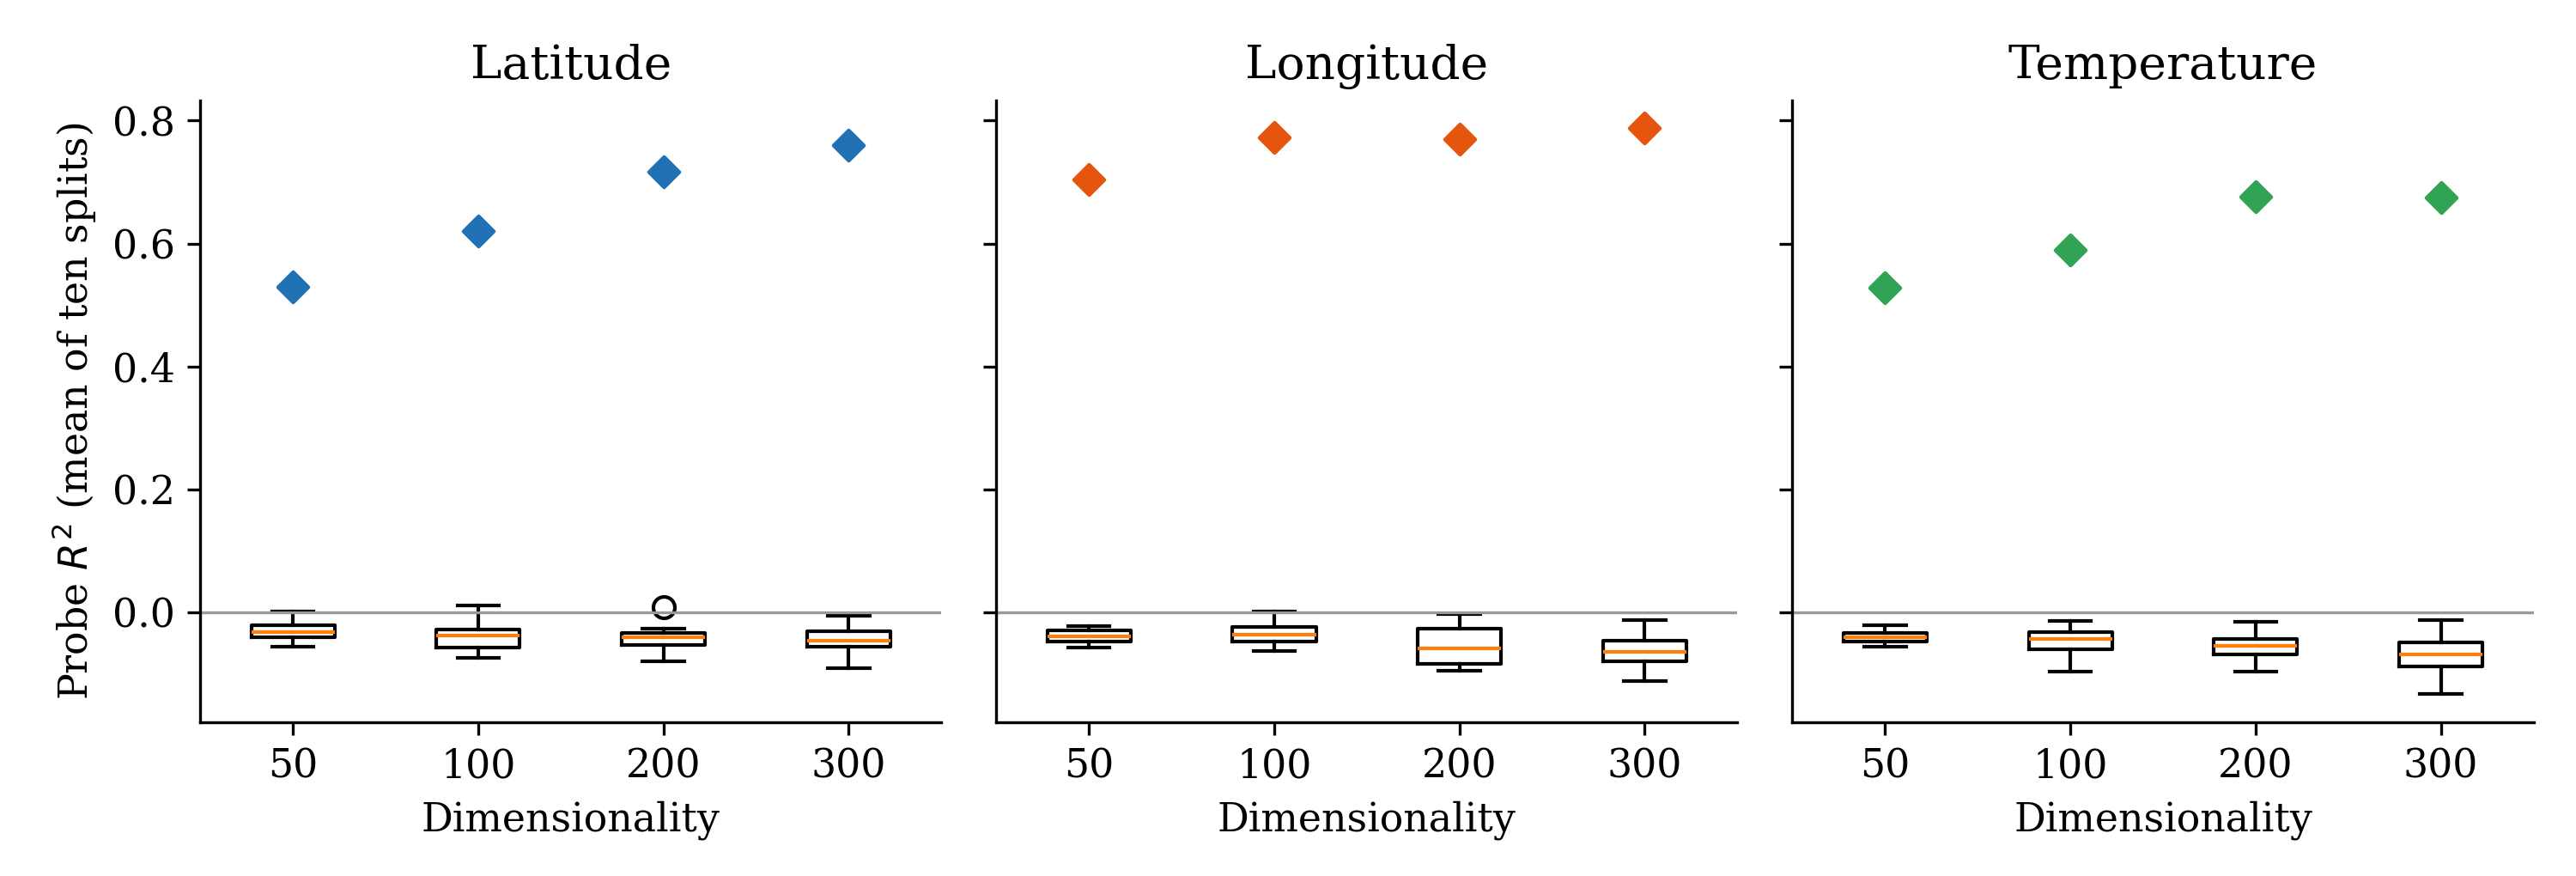
\includegraphics[width=\textwidth]{fig_random_control.png}
  \caption{Random embedding control. Box plots show the ten-split mean probe $R^2$ for each of 20 sets of random Gaussian vectors at each dimensionality. Colored diamonds show corresponding GloVe $R^2$ values. The probes find no structure in random embeddings at any dimensionality.}
  \label{fig:randomcontrol}
\end{figure}

\subsection{Semantic Similarity Analysis}
\label{sec:semantic}

The preceding results establish that static embeddings preserve substantial spatial and temporal structure. We next ask whether this structure is semantically interpretable: does the embedding space encode geography through co-occurrence with meaningful vocabulary, and if so, which words carry the signal?

\paragraph{Data-driven word correlations.}
Rather than selecting probe words \textit{a priori}, we take a data-driven approach. For every word in the GloVe vocabulary (restricted to the 20,000 most frequent words with at least four letters, excluding the cities' own name words and a list of common country names, demonyms and geographic terms; other proper nouns, such as \emph{mozambique} or \emph{nikolai}, remain), we compute its cosine similarity to each of the 272 city embeddings, producing one similarity value per city. We then correlate these 272 similarity values with the cities' actual mean annual temperatures (Pearson $r$). Figure~\ref{fig:semantic_spatial} shows the 15 most positively and 15 most negatively correlated words.

Both directions are semantically interpretable. Words most associated with warmer cities reflect tropical ecology and disease burden---``dengue'' ($r = +0.61$), ``malaria'' ($r = +0.59$), ``jungle'' ($r = +0.56$), ``crocodile'' ($r = +0.52$), ``cyclone'' ($r = +0.52$), ``mosquito'' ($r = +0.50$), ``cholera'' ($r = +0.48$). Words most associated with colder cities reflect winter activities and European cultural institutions---``skaters'' ($r = -0.57$), ``skating'' ($r = -0.56$), ``philharmonic'' ($r = -0.53$), ``violinist'' ($r = -0.53$), ``orchestra'' ($r = -0.52$), ``conservatory'' ($r = -0.51$), ``skiing'' ($r = -0.50$), ``conductor'' ($r = -0.50$).

These semantic categories were not selected \textit{a priori}; they emerge from an exhaustive search over the vocabulary. Because the reported words are selected for having large correlations, we treat the rankings as exploratory and report no inferential test on them. The results confirm that the embedding space encodes temperature through graded co-occurrence with climatically and culturally relevant vocabulary.

\paragraph{Shared company.}
To see why a city name's representation is similar to those of words such as
\emph{malaria} or \emph{orchestra}, we ranked each of the 50{,}000 most frequent GloVe words
by its similarity to the mean representation of the names of the 25 warmest (or coldest)
of our cities, taken relative to the mean over all cities, and separately by its similarity
to the anchor words, and took the words that rank high on both. For warm cities and
\emph{malaria} and \emph{jungle}, these are mostly Southeast Asian place names and tropical
landscape (\emph{jungles}, \emph{borneo}, \emph{cambodia}, \emph{laos}, \emph{mekong},
\emph{thailand}). For cold cities and \emph{skiing}, they are winter sports and Nordic places
(\emph{hockey}, \emph{lillehammer}, \emph{rink}, \emph{finland}, \emph{nordic}); for cold
cities and \emph{orchestra}, Russian classical music and its institutions (\emph{bolshoi},
\emph{prokofiev}, \emph{kirov}, \emph{leningrad}, \emph{shostakovich}, \emph{tchaikovsky}).
Words for the weather rank far lower: \emph{humid}, for example, ranks below 20{,}000th in
similarity to the warm cities' names.

For the released historical figures the same search is dominated by the makeup of the
names rather than by period vocabulary: the words whose similarity to the representations of
the figures' names best tracks year of death are Chinese provinces and cities (earlier; e.g.\ ``henan'', ``guangdong'', $r
\approx -0.49$) and modern Western given names and surnames (later; e.g.\ ``wally'',
``carlson'', $r \approx +0.45$), along with occupations such as ``chemist'' and
``biologist''. The temporal signal in the static vectors comes largely from where, and in what
roles, people are written about.

\paragraph{Composite scores.}
The preceding analysis shows that geographic signal is distributed across many words in the vocabulary. A complementary question is how little information is needed: can just two well-chosen words capture the signal?

Composite scores constructed from antonym pairs suggest that they cannot. The cold--warm composite---defined as cosine similarity to ``cold'' minus similarity to ``warm'' for each city---correlates with latitude at only $r = 0.41$ and with temperature at $r = -0.34$.
For the released historical figures, a modern--ancient composite correlates with year of
death at only $r = 0.23$, consistent with the name-driven structure described above.
Together with the data-driven analysis, these results indicate that the signal is distributed across much of the vocabulary rather than concentrated in the words for the property itself.

\subsection{Semantic Subspace Ablation}
\label{sec:ablation}

Table~\ref{tab:ablation} reports the $R^2$ drop for each semantic category when its subspace
is removed from the GloVe city embeddings, and its $z$-score against random word sets matched
on number of words, frequency, proper-name status, vector norm and dimensionality
(Appendix~\ref{sec:ablation_methods}). Baseline (unablated) $R^2$ values are $0.760$ for
latitude, $0.788$ for longitude and $0.675$ for temperature.

\begin{table}[t]
  \centering
  \caption{Semantic subspace ablation (272 cities, GloVe). $\Delta R^2$: drop in ten-split
  mean $R^2$ when a category's subspace is removed. $z$: the drop against 200 random word
  sets matched on number of words, frequency, proper-name status, vector norm and
  dimensionality; $^{*}$ marks an empirical one-sided $p \leq .01$ ($1/201$ is the smallest
  attainable). The last column is the share of the city embeddings' variance the subspace
  removes, with the mean over the matched sets in brackets.}
  \label{tab:ablation}
  \footnotesize
  \setlength{\tabcolsep}{4pt}
  \begin{tabular}{lccccccccc}
    \toprule
    & & \multicolumn{2}{c}{Latitude} & \multicolumn{2}{c}{Longitude} & \multicolumn{2}{c}{Temperature} & City variance \\
    \cmidrule(lr){3-4} \cmidrule(lr){5-6} \cmidrule(lr){7-8}
    Category & Dims & $\Delta R^2$ & $z$ & $\Delta R^2$ & $z$ & $\Delta R^2$ & $z$ & removed \\
    \midrule
    Country names        & 20 & $+0.226$ & $3.3^{*}$ & $+0.155$ & $2.0$ & $+0.224$ & $3.2^{*}$ & .29 (.24) \\
    Region \& continent  & 18 & $+0.119$ & $2.3$     & $+0.011$ & $-1.6$ & $+0.063$ & $0.7$ & .16 (.17) \\
    Climate \& weather   & 19 & $+0.048$ & $4.0^{*}$ & $+0.007$ & $0.0$ & $+0.090$ & $7.7^{*}$ & .12 (.11) \\
    Cultural \& language & 20 & $+0.031$ & $-0.4$    & $+0.026$ & $-0.7$ & $+0.067$ & $0.7$ & .20 (.18) \\
    Cardinal directions  & 9  & $+0.018$ & $0.6$     & $+0.007$ & $-0.9$ & $+0.021$ & $1.3$ & .07 (.08) \\
    Economic terms       & 19 & $+0.004$ & $-0.3$    & $-0.000$ & $-1.0$ & $+0.015$ & $0.8$ & .11 (.10) \\
    \bottomrule
  \end{tabular}
\end{table}

Against matched word sets, three results stand out. Removing \textbf{climate and weather}
terms costs temperature far more than matched vocabularies do ($\Delta R^2 = 0.090$,
$z = 7.7$), and latitude somewhat more ($z = 4.0$), but leaves longitude where matched sets
do ($z = 0.0$), although these terms remove no more of the city embeddings' variance than
the matched sets. \textbf{Country names} produce the largest decrement on every target and
exceed the matched sets for latitude and temperature ($z = 3.3$ and $3.2$); their subspace
also aligns more closely with the city vectors than any matched set (29\% of the city
variance against $24 \pm 1$\%). Regressing the matched sets' decrements on the share of city
variance they remove and extrapolating to the country subspace's share predicts decrements of
$0.15$--$0.16$, which matches the longitude decrement and accounts for 35--43\% of the excess
on latitude and temperature; because the country subspace lies outside the range of the
matched sets, this attribution is approximate. \textbf{Region and continent} names
exceed the matched sets only for latitude ($z = 2.3$, $p = .03$). The remaining vocabularies
(cultural and language terms, cardinal directions and economic terms) cost no more than
matched random words. Against random orthonormal subspaces, the comparison used in an
earlier version of this analysis, every category except economic terms appeared to have a
large effect ($z$ up to 42); most of that reflected the weakness of that null rather than
anything specific to the vocabularies.

The data thus indicate that what the probes use is concentrated in directions shared with
country names, and, for temperature, with words for climate and weather, in line with the
word correlations above. Two limits should be stated. The ablations remove directions in
embedding space; they are not interventions on the corresponding words in the training
corpus, and each subspace may carry correlated information from several sources, so the
individual drops are not additive contributions. And the category labels describe the
vocabulary used to construct each subspace, not the content the subspace is thereby shown to
contain.

\end{document}
